\chapter{Dynamic Molecular Docking}

This chapter is a customized version of \cite{dmd_samsonov_gehrcke_2014}, where
we have published the description and validation of Dynamic Molecular Docking.

% American Chemical Society’s Policy on Theses and Dissertations
% http://pubs.acs.org/userimages/ContentEditor/1218205107465/dissertation.pdf

\section{Abstract}
We present Dynamic Molecular Docking (DMD), a novel
targeted molecular dy\-namics-based protocol developed to address ligand and
receptor flexibility as well as the inclusion of explicit solvent in local
molecular docking. A class of ligands for which docking performance especially
benefits from overcoming these challenges are glycosaminoglycans (GAGs). GAGs
are periodic, highly flexible and negatively charged polysaccharides playing an
important role in the extracellular matrix via interaction with proteins such as
growth factors and chemokines. The goal of our work has been to develop a proof
of concept for an MD-based docking approach and to analyze its applicability for
protein-GAG systems. DMD exploits the electrostatics-driven attraction of a
ligand to its receptor, treats both as entirely flexible and considers solvent
explicitly. We show that DMD has high predictive significance for systems
dominated by electrostatic attraction and demonstrate its capability to reliably
identify the receptor residues contributing most to binding.

\section{Rational}

Molecular docking has been extensively applied for drug
discovery in the recent decades \cite{klebe_recent_2000,
cheng_structure-based_2012}. Whereas molecular docking methodologies demonstrate
to be very successful and continue to develop rapidly, they still suffer from a
number of limitations \cite{moreira_proteinprotein_2010,
andrusier_principles_2008,lensink_docking_2010}. What holds true for practically
all docking methods is that the reproduction of an experimentally observed
docking pose is less challenging than proper scoring of this pose by energy
\cite{kim_assessment_2008, plewczynski_can_2011,smith_csar_2011}. In the
majority of docking approaches, only small ligands can be treated as entirely
flexible in order to limit the size of the conformational search space. Although
flexible treatment of the ligand is crucial for obtaining meaningful results,
ligand flexibility often can only be approximated, especially in protein-protein
docking \cite{ritchie_recent_2008}. Another severe approximation applied in most
docking methods is static treatment of the receptor even though protein side
chain flexibility is crucial for ligand binding, and substantial conformational
changes can occur in the receptor structure induced by interaction with a ligand
\cite{gunasekaran_how_2007,gutteridge_conformational_2005}. Finally, most of the
established docking approaches do not explicitly account for solvent molecules,
whereas many studies point out their importance in docking calculations
\cite{van_dijk_solvated_2006,baron_water_2010,roberts_ligandprotein_2008,
thilagavathi_ligand-protein_2010}.

A particularly challenging class of ligands for which docking
performance is especially limited by the above-mentioned issues are
glycosaminoglycans (GAGs), which are periodic negatively charged linear
polysaccharides mainly located in the extracellular matrix. Through interaction
with their protein targets they participate in a number of key processes
involved in cell regeneration and proliferation, angiogenesis, metastasis and
lipid metabolism \cite{hynes_extracellular_2009, macri_growth_2007,
barbero_chembiochem_2013}. Due to the occurrence of numerous sulfate and
carboxyl groups, GAGs have a high charge density, rendering long-range Coulomb
interaction to be crucial for binding to proteins
\cite{mulloy_specificity_2005}. The significance of electrostatic interaction
underlines the importance of taking explicit solvent molecules as binding
mediators into account when GAGs are used as ligands in molecular docking
\cite{samsonov_docking_2011}. Moreover, the orientation and conformation of long
side chains of charged protein residues may be greatly influenced by interaction
with a GAG ligand. In consequence, flexible treatment of the receptor during
GAG-docking is of special relevance. In addition, a similar spatial distribution
of functional groups in GAGs independent of the reducing/non-reducing end
orientation \cite{hp_binding_sites_mulloy_2006} as well as their high
flexibility \cite{bitomsky_docking_1999} substantially contribute to the
challenges in protein-GAG docking. Overall, the prediction of protein-GAG
complexes via molecular docking comprises a good example of some of the current
limitations in the field of classical molecular docking.

Classical docking approaches are generally optimized for having relatively
modest computational requirements and therefore enable the quick investigation
of single complexes as well as the execution of large-scale studies involving a
large number of different complexes. Taking into account ligand and receptor
flexibility as well as treating solvent explicitly clearly increases the
computational complexity of docking approaches. However, in view of the
ever-increasing computing power, a new generation of docking methods should
evolve, which though being computationally more demanding, aims to deal with the
above-mentioned challenges.

Molecular dynamics (MD) techniques are established for rigorous studies of
intermolecular interactions \cite{karplus_molecular_2005}. Beyond that, MD
methods have already been used in docking approaches for overcoming the
challenges of both ligand and receptor flexibility
\cite{chaudhuri_application_2012, antes_dynadock_2010}. Furthermore, standard MD
methods allow for the inclusion of explicit solvent via well-established water
models. The application of MD techniques is limited by high computational cost,
which previously has hindered their usage in high-throughput approaches for drug
discovery. However, nowadays, advanced computational resources are available and
specialized hardware (such as graphics processing units, GPUs) can be used to
dramatically increase the performance of MD simulations, making the
establishment of MD in the field of docking gradually feasible.

We propose Dynamic Molecular Docking (DMD), a combination of established
MD-based methods specifically designed for tackling the above-mentioned
challenges in protein-GAG docking. DMD is a targeted MD-based approach where the
ligand, which is initially placed at a distance from the receptor so that their
interaction is negligible, is slowly pulled towards a receptor target region by
applying a time-dependent distance restraint. During this process, both receptor
and ligand are treated as entirely flexible in explicit solvent. The time-
dependent distance restraint applied in DMD is usually used in steered molecular
dynamics simulations, which are performed for studying the energetics of
processes that generally happen on timescales too large for being treated by
classical MD simulations \cite{xiong_free_2006}, such as protein folding, ligand
unbinding and large-scale conformational alteration. In DMD, once the ligand
reaches the receptor, the distance restraint is switched off and a long free MD
simulation is carried out, allowing for the mutual adjustment of receptor
residues and GAG as well as for extensive GAG-internal degree of freedom
sampling. The obtained trajectory data are then used for \textit{i)} extracting
a docking solution (the coordinates of the ligand relative to the receptor) and
\textit{ii)} for the characterization of this docking solution. In terms of
molecular docking, this method keeps binding pose search well as binding pose
scoring consistent, in the sense that both use the same potential as given by
the MD force field and the parameterization of the molecular system.

Classical molecular docking is usually based on a phenomenological model,
whereas the internal parameters have been trained based on a set of molecular
reference systems (often, machine learning tools are applied for this task).
This raises the question about the applicability of such model to systems
outside the training data set, and about the validity of the resulting data. In
contrast, one of the main conceptual advantages of molecular dynamics
simulations compared to classical docking approaches is that the underlying
model and its parameters are (classical) physics-based. The parameters have been
developed over years with the goal to make dynamics simulations reproduce the
classical chemical and physical properties of the simulated system. Hence, if
properly set up, MD simulations produce data that is generally more trustable
and resilient than data produced by machine learning-based docking methods.

One of the main concepts of a DMD study is that pulling process and subsequent
free MD are repeated \textit{many} times in independent simulations. This allows
for the creation and evaluation of an ensemble of docking solutions rather than
the interpretation of single trajectories. In this ensemble, the energetically
more favorable states are the more likely ones. Subsequent spatial clustering of
this docking solution ensemble identifies those docking solutions that appeared
with highest probability and, therefore, lowest energy. We should note that a
meaningful DMD study requires a reasonable assumption about the binding region
it is focused on. However, there is no general dependence of the DMD protocol on
the confidence in the binding region assumption --- selection of the binding
region and local docking are independent tasks.

\begin{figure}
\centering
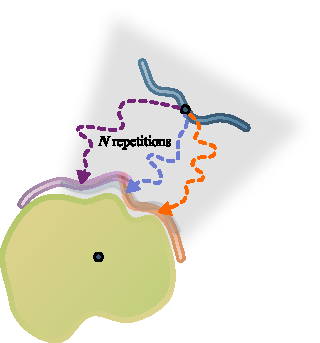
\includegraphics[height=7cm]{gfx/dmd/scheme_n_repetitions_for_thesis_002.pdf}
\caption[]{Schematic representation of the DMD pulling process. Starting from a
distal position, the ligand (blue) is pulled towards its receptor (green).
During this process, the ligand moves along a random path. The pulling process
is repeated $N$ times in independent simulations. Most of the resulting ligand
trajectories lie within a certain \enquote{entry lane}, as depicted here in grey
shade. Each pulling process yields an individual final ligand state (purple,
blue, orange) near the receptor surface.}
\label{fig:dmd:n_repetitions}
\end{figure}


\section{General method description}
\subsection{Data production}

A DMD study for a given receptor-ligand complex implies performing $N$ (e.g.
100) independent DMD runs. The number of independent repetitions $N$ must be
large enough for obtaining convergence regarding certain ensemble properties.
Each DMD run starts with a randomly oriented ligand molecule placed at a
distance from the receptor (ligand re-oriented model, LROM). The first step of a
DMD run is a targeted molecular dynamics (tMD) simulation in which the ligand is
pulled towards a pre-defined target region on the receptor via a time-dependent
decrease of the distance $d(t)$ between one central atom in the ligand and one
core atom in the protein receptor. Among DMD run repetitions, most of the ligand
trajectories lie within a certain \enquote{entry lane} which is focused on a
point near the receptor surface, the focus point $\bm{F}$, and therefore
defining the target region (\cref{fig:dmd:n_repetitions}). All final tMD states
have the central ligand atom positioned on the surface of a sphere defined by
the protein core atom (the center of the sphere) and the final distance $D$ of
the tMD pulling process (the radius of the sphere). Based on the final state of
each tMD simulation, the second step of a DMD run relaxes the system via a free
MD simulation. Geometrical definitions, system preparation, and details about
tMD and free MD parameterization as well as subsequent trajectory data analysis
methods are provided in the following sections.

\begin{figure}
\centering
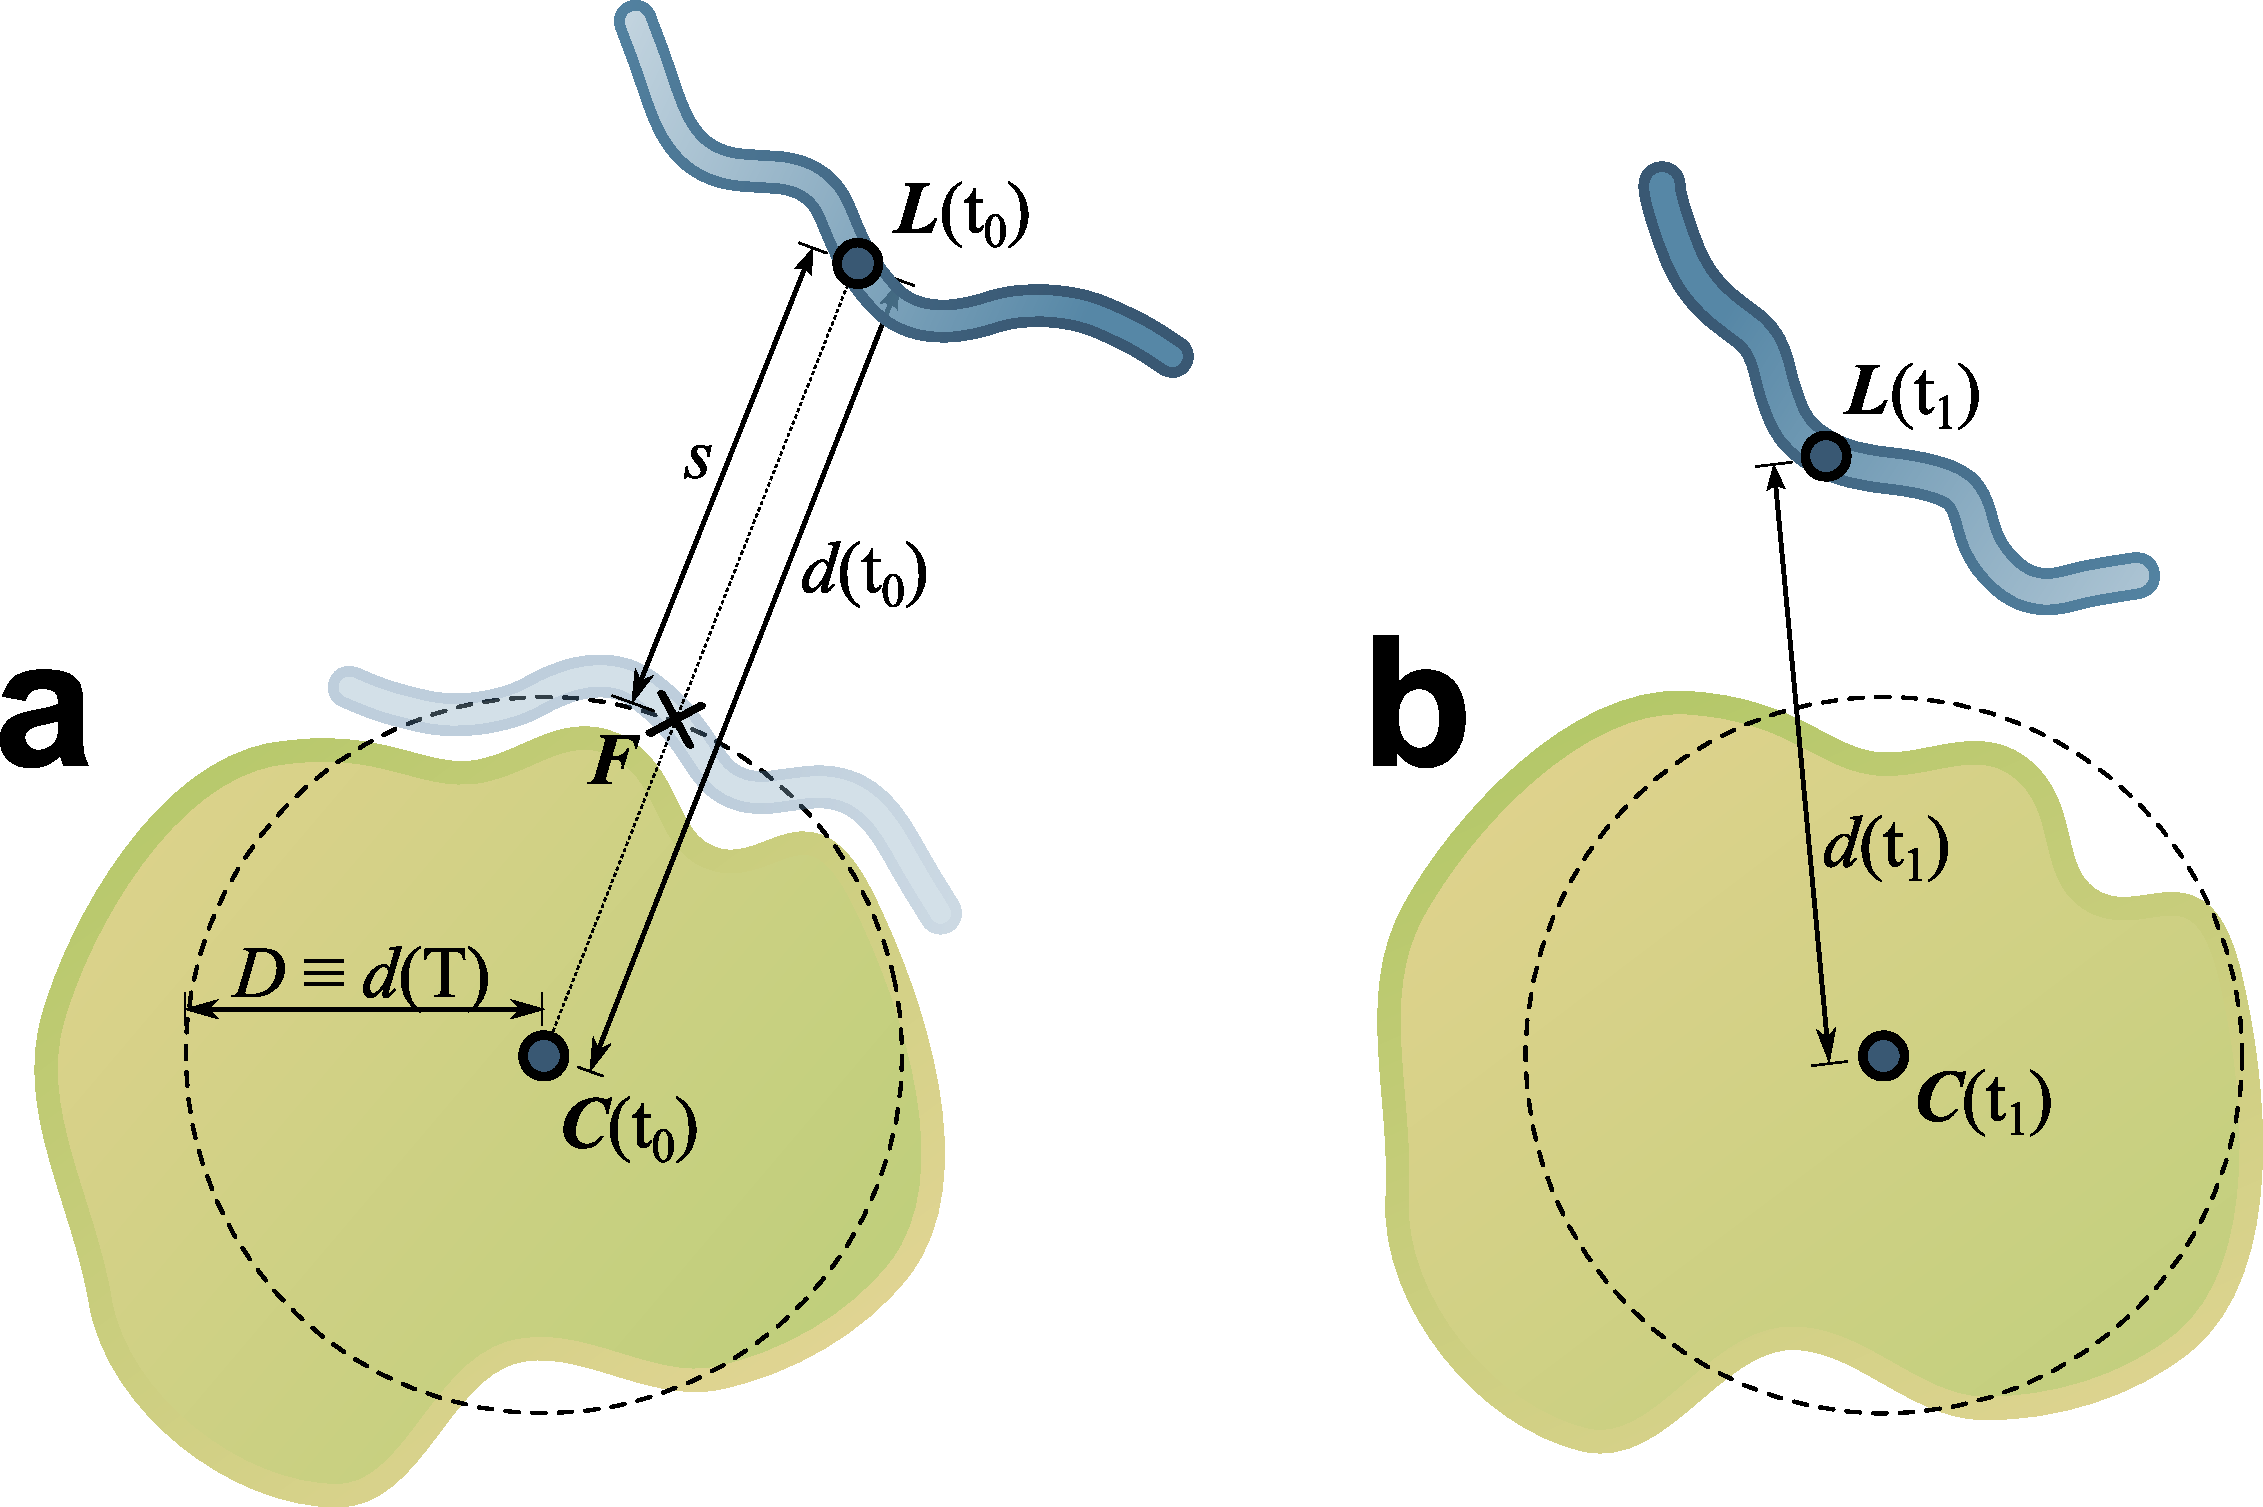
\includegraphics[height=7cm]{gfx/dmd/scheme_geometry_two_panels_002.pdf}
\caption[]{
\textbf{a}: System configuration at time $t_0$ right before the pulling process,
referred to as the ligand-reoriented model (LROM, with the displaced ligand in
dark blue). The central atom of the experimentally determined ligand position
(light blue) has been placed to a distal position $\bm{L}(t_0)$ along the axis
given by a receptor core atom at point $\bm{C}(t_0)$ and the focus point
$\bm{F}$. $s$ is the displacement length. The ligand has been randomly rotated
around its central atom. The distance between $\bm{C}(t_0)$ and $\bm{F}$ defines
the final distance $D$ for the ligand pulling process. The initial distance
$d(t_0)$ between $\bm{C}$ and $\bm{L}$ is $D+s$.
\textbf{b}: arbitrary state within the pulling process, during which the
distance $d(t)$ between central ligand atom at point $\bm{L}(t)$ and protein
core atom at point $\bm{C}(t)$ is decreased over time $t$. Right after the
pulling process, all final ligand states have their central atom placed on the
sphere that is indicated here with a dashed line.
}
\label{fig:dmd:geometry_scheme}
\end{figure}

\subsubsection{Preparation of ligand-reoriented models (LROMs)}
An LROM contains
the receptor as well as the ligand placed in a distal, re-oriented position. Per
TDS complex, ten LROMs have been created, differing only in ligand orientation
around its central atom. For a given complex, LROM creation requires the
selection of a \textit{central ligand atom}, definition of a \textit{focus
point} $\bm{F}$ near the surface of the receptor within the anticipated binding
region, definition of a \textit{ligand displacement length} $s$ and selection of
a \textit{core atom} at point $\bm{C}$ within the receptor. The distance between
focus point and core atom defines the final distance $D$ of the tMD pulling
process, i.e.\  $d(T) \equiv D \equiv  \lVert \bm{F}-\bm{C} \rVert$. Initially,
at time $t_0$, the ligand is placed distal from the receptor with its central
atom lying on the axis defined by $\bm{F}-\bm{C}$
(\cref{fig:dmd:geometry_scheme}a). The starting coordinate for the central
ligand atom is defined as

\begin{equation}
\bm{L}(t_0) = \bm{F} + s \frac{\bm{F}-\bm{C}}{D}.
\end{equation}

For each TDS complex, multiple LROMs should be prepared as follows. First, the
structure of the biological unit of the protein receptor is to be taken from the
corresponding experimental data source (3D structure from crystallography or
NMR). The coordinates of a central atom in the ligand as found in the
experimentally determined structure are to be used as focus point. The core atom
in the receptor must be selected fulfilling three criteria: \textit{i)} it is a
backbone atom within a helix or beta sheet in the protein core, \textit{ii)} the
line connecting core atom and $\bm{F}$ (defining the orientation of the ``entry
lane'' is roughly perpendicular to the surface comprising the anticipated
binding region, and \textit{iii)} the surface of the sphere around the core atom
with radius $D$ has significant overlap with the molecular receptor surface in
the receptor target region. Distal ligand placement is to be followed by
multiple random ligand rotations uniformly distributed in 3D space with
$\bm{L}(t_0)$ being the rotation center. Each rotational ligand corresponds to
one LROM.

\subsection{Data analysis}

MD simulations provide a plethora of data extraction and analysis possibilities,
and in general the researcher is not limited in his/her creativity to extract
interesting quantities from the raw data of a DMD study. Namely, the available
raw data are the trajectories of $N$ tMD and $N$ free MD simulations, which in
total usually comprise one or more microsecond(s) of simulated real time. In
this section, we provide an overview about how DMD data analysis should be
performed in general, classify the different approaches, and discuss some
obvious data extraction techniques.

\begin{figure}
\centering
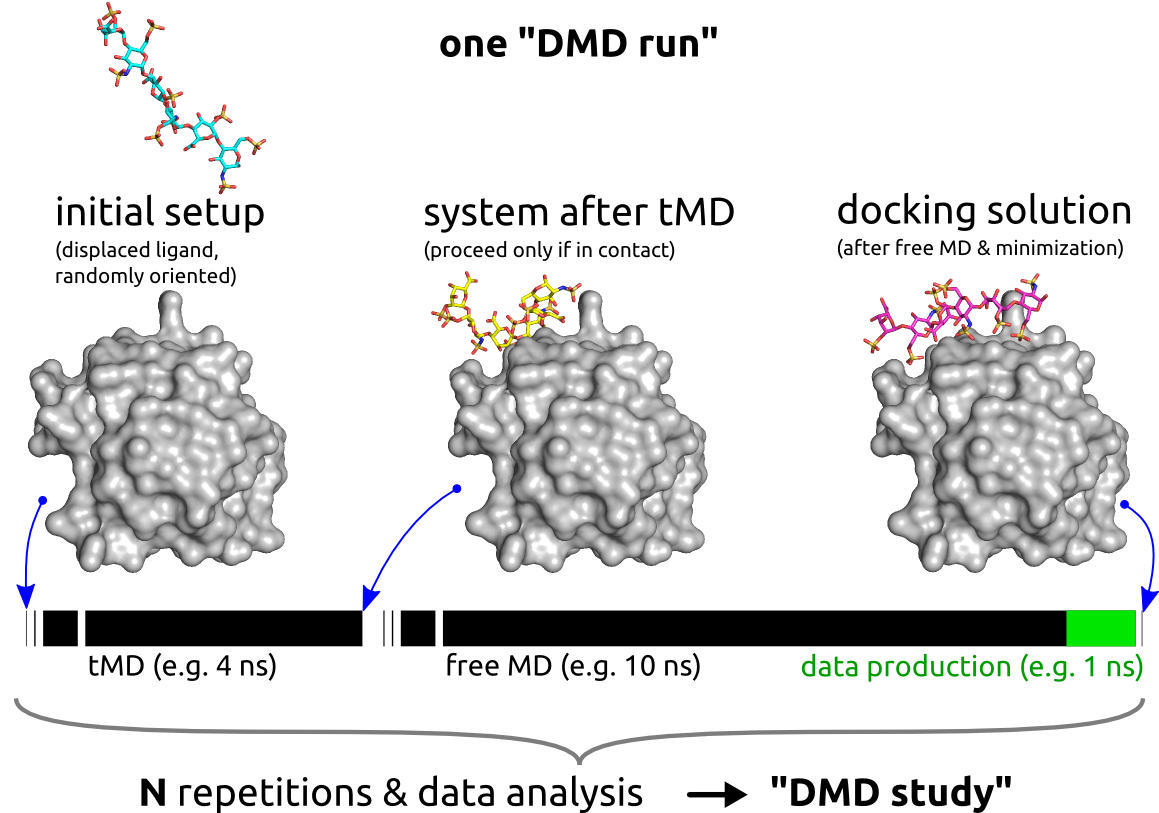
\includegraphics[width=1.0\textwidth]{gfx/dmd/dmd_timeline_for_thesis_09.png}
\caption[]{
Schematic overview of the chronological sequence of a DMD run, and definition of
the term \enquote{DMD study}. The black bars, read from left to right, provide
an overview of the time course of a single DMD run: its starts off with the
initial system (example system shown at the left, with the protein surface in
gray and the ligand shown in blue sticks) and proceeds with the targeted
molecular dynamics (tMD) process. The final tMD system state (central example
system with the ligand shown in yellow sticks) is further processed in a free MD
simulation. tMD and free MD involve the usual MD preparations (minimization,
heat-up, and equilibration), as indicated by the shorter black bars. The
coordinates of a single docking solution are the result of energy minimization
of the final free MD state (example system on the right, with the ligand shown
in magenta sticks). Extraction of data for docking solution characterization is
limited to the final fragment of free MD, as indicated in green.}
\label{fig:dmd:timeline}
\end{figure}


First of all, we need to clarify which fractions of the trajectories of a DMD
study are interesting for data extraction. Method characterization for sure
requires analysis of all trajectory data created. Application of the method,
however, focuses on docking solution \textit{generation} and
\textit{characterization}. For this task, it is required to ignore most parts of
the trajectory data, namely the entire tMD process as well as the first major
part of the free MD simulations. These parts are strongly relevant for sampling,
they however are not applicable for characterizing the final state of a DMD run,
i.e.\ the \textit{docking solution} corresponding to that run. That is why we
have (arbitrarily) decided to use the last \SI{1}{\nano\second} of the free MD
simulation, for extracting data about a single docking solution. For
clarification, \cref{fig:dmd:timeline} shows the relation of a \enquote{DMD
study} and single \enquote{DMD runs}, as well as a time line of a single DMD run
with specific labeling of the time interval relevant for data extraction.

\subsubsection{Characterization of single docking solutions}

Conceptually, data extraction is performed for single DMD runs. That is,
evaluation of the tail of any given free MD simulation yields certain
quantities, and these quantities correspond to one DMD run only. Such quantities
can be used for characterizing the single docking solution as obtained from that
DMD run. These quantities can be classified as either of \textit{static}, or of
\textit{dynamic} nature. Static quantities are derived from the energy-minimized
free MD final system state, i.e.\ from \textit{one} set of coordinates only.
Meaningful examples of such static quantities are:

\begin{itemize}
\item The minimal distance between receptor and ligand, i.e.\ the distance
between those two atoms in receptor and ligand which are closest to each other
of all receptor-ligand atom pairs. This quantity describes whether receptor and
ligand are in contact or not. An atomic contact in an organic system usually
leads to an inter-atomic distance of slightly below \SI{2}{\angstrom}.
\item The average minimal distance between receptor and ligand, i.e.\ find the
closest atom in the receptor for each atom in the ligand and build the mean of
all resulting atom pair distances. For ligand molecules such as GAGs this
quantity describes the alignment of receptor and ligand: a small value suggests
that the ligand is entirely aligned with the receptor. A large value on the
other hand means that most parts of the ligand are not in contact with the
receptor.
\end{itemize}

These quantities can be convenient for automatically filtering DMD runs, e.g.\
for separating out those docking solutions where receptor and ligand are not in
contact with each other, by pure geometric criteria. Dynamic quantities on the
other hand implicate analysis of multiple MD trajectory frames. That is, they
are based on multiple sets of coordinates that represent the \textit{dynamic}
nature of the system as simulated by the MD method. Meaningful examples of such
dynamic quantities are:


\begin{itemize}
\item The internal ligand flexibility, measured in \si{\angstrom}. Can be
calculated by iterating through the MD frames while aligning the ligand
coordinates of the current frame to those in the first frame, and then building
the root mean square distance ($RMSd$) for all MD frames in question,
yielding a time series of $RMSd$ values. The standard deviation of this time
series represents the fluctuation of the data, i.e.\ the internal ligand
flexibility.

\item The mobility of the ligand relative to the receptor, measured in
\si{\angstrom}. The procedure is the same as described before, with the
difference that the receptor is aligned to the receptor prior to measuring the
$RMSd$, i.e.\ the receptor defines the reference coordinate system, and not the
ligand. Hence, the standard deviation of this $RMSd$ time series represents the
overall mobility of the ligand with respect to the receptor.

\item The average number of hydrogen bonds established between ligand and
receptor. For simple analyses, it is safe and established to infer hydrogen
bonds by simple atom type, distance, and angle criteria
\cite{hbonds_crystal_survey,hbonds_sulfur_1991}, as implemented in the MD
trajectory analysis software cpptraj \cite{cpptraj_2013}. The average number of
hydrogen bonds throughout the tail of the free MD trajectory gives quite useful
clues about how many high affinity atomic contacts are established in the
binding mode described by the docking solution. The and the corresponding
standard deviation of this time series expresses the stability of the hydrogen
bonding network.

\item Hydrogen bonds can also be analyzed by tracking the existence of specific
acceptor-donor atom pairs over time, which allows for determination of the time
fraction of occupancy of such a specific pair. Acceptor-donor atom pairs can
then be ranked by their relative occupancy, in order to determine the importance
of single hydrogen bonds.

\item Hydrogen bonding can also be analyzed by tracking the occupancy of single
donors or acceptors over time, yielding the importance of single atoms in the
ligand or atoms/amino acid residues in the protein receptor.

\item Estimation of the free energy of binding via end-point free energy methods
such as MM-PBSA or MM-GBSA (cf. \cref{methods:mmpbsa_mmgbsa} \hl{CHECK CREF}).
These methods are usually applied to a time series of MD trajectory frames, and
yield an estimate for the contributions of different interaction types to the
overall binding affinity, including standard deviation and standard error of the
mean. Different docking solutions of the same molecular system can be ranked by
such free energy of binding estimates, providing a meaningful and convenient
tool for comparison among different docking solutions.

\item So-called single-residue energy decomposition (SRED) can be performed via
a specialized form of the MM-GBSA analysis (cf. \cref{methods:mmpbsa_mmgbsa}
\hl{CHECK CREF}). SRED assigns an energy value for each amino acid residue in
the protein receptor and therefore enables meaningful ranking of such residues
by importance for ligand binding.
\end{itemize}


\subsubsection{Merge the data: extraction of ensemble properties}

We have stressed before that an essential concept of DMD is the creation and
analysis of an entire \textit{ensemble} of docking solutions. In fact, the
characterization of single docking solutions does not necessarily yield
trustable or even meaningful insights about the protein-ligand system under
investigation. The ensemble properties, however, are assumed to be
\textit{converged}, i.e.\ an independent repetition of the same DMD study would
yield different individual docking solutions, but ensemble properties of the
same kind. As of the validity of the underlying model, a converged result of MD
simulations is usually \textit{reliable} and \textit{meaningful}. Therefore, we
seek to extract ensemble properties of a DMD study. \textit{Static}
coordinate-based docking solution ensemble evaluation by means of clustering has
been discussed before in \cref{chapter:clustering}. Here, we describe an
additional approach for extracting \textit{dynamic} DMD study ensemble
properties that are likely to provide essential insights about the molecular
system under investigation.

Two of the single docking solution analysis types listed above are qualified for
\textit{merging} their results among (nearly) \textit{all} docking solutions:
hydrogen bonding occupancy analysis and single-residue energy decomposition. The
idea behind such data merge operation is to find those residues in the protein
receptor that are most important for ligand binding, whereas the entire DMD
study provides the corresponding data, rendering the outcome significant and
trustable. Essentially, the merge operation is comprised of \textit{filtering}
useful docking solutions, and \textit{averaging} their corresponding quantities
for single residues in the protein receptor. The filtering step makes sure that
no invalid (e.g.\ unbound) docking solutions contribute to the final result. The
averaging operation merges the ensemble data, enriched with statistics: it
usually makes sense to track standard deviation and standard error of the mean
in order to decide whether the merge provides valid data or not. The result of
the merge is an \textit{ensemble-derived quantity} for each protein residue.
Obviously, the average of a certain quantity measured for a \textit{diverse} set
of docking solutions does not provide a meaningful absolute value. The merge
operation, however, provides a meaningful \textit{ranking} among the different
protein residues. Simply spoken, this kind of analysis helps identifying those
residues that are most important for binding in most of the single DMD runs ---
just in a systematic and reliable way.


\section{DMD implementation for this thesis project}

\subsection{Molecular dynamics protocol}

The DMD-related molecular dynamics simulations performed in the context of this
PhD project were set up, performed, and analyzed using Amber 12 and AmberTools
12 \cite{case_amber_11}. The FF99SB force field was used for parameterization of
the peptidic parts in the investigated complexes. GAG force field parameters
were created based on GLYCAM 06 version g \cite{kirschner_glycam06:_2008} and
sulfate partial charges obtained by RESP fitting calculations at the level of
6-31(d)G for methylsulfate. All systems were solvated in a box of TIP3P water
with a minimum of \SI{8}{\angstrom} distance between solute and box boundaries.
The systems were neutralized by adding Na$^{+}$ or Cl$^{-}$ counterions. The MD
time integration step was set to \SI{2}{\femto\second}, whereas bonds including
hydrogen atoms were length-constrained by the standard SHAKE method. During MD,
non-bonded interactions were switched off for atom pairs further apart than
\SI{8}{\angstrom}. The Particle Mesh Ewald method was used for treating
long-range electrostatic interactions.

Each simulated system went through minimization, heat-up, equilibration, and
production steps. During the first stage of minimization, only the solvent was
relaxed. During the second stage, the entire system was minimized without
restraints. System heat-up to \SI{300}{\kelvin} was performed within
\SI{20}{\pico\second} of simulated real time in the canonical ensemble (NVT)
using the Langevin thermostate and periodic boundary conditions. Subsequently,
\SI{500}{\pico\second} of MD in the isothermal-isobaric ensemble (NPT) with
Langevin thermostate and Berendsen barostat under periodic boundary conditions
were carried out for system density equilibration. The following production
stage of duration $T$ was performed in the NVT ensemble with the Berendsen
thermostat and periodic boundary conditions.

%For complexes involving heparin, weak torsional restraints were
%applied in order to keep the pyranose rings of IdoA(2S) in the $^{1}C_4$
%conformation. This conformation has been shown to be one of the two
%predominantly populated ones{\cite{almond_jacs_2010}} and was observed
%experimentally in the structure of the FGF2-HP complex in our test data set (PDB
%ID 1BFB). The applied restraints enable to define and control the specific
%%conformation of each IdoA(2S) ring throughout the entire DMD study, since its
%natural ring conformer population is not properly reproduced by GLYCAM
%06{\cite{gandhi_idoa2s_2010}}.

\subsubsection{Targeted and free molecular dynamics.}
The LROMs were prepared for MD and time-evolved following the general MD
protocol as described above. During the tMD production stage, core atom and
ligand center atom were exposed to an additional time-dependent harmonic
potential

\begin{equation}
U(t) = \frac{1}{2} k \left( d(t)-d(t_0) + vt   \right)^2
\end{equation}

with force constant $k=200\,\mathrm{kcal\,mol^{-1}\,A^{-2}}$, pulling velocity
$ v = s/T$ and

\begin{equation}
d(t) = \lVert \bm{L}(t)-\bm{C}(t) \rVert.
\end{equation}

This potential enforces the distance between the selected ligand center atom and
the protein core atom to linearly decrease with time $t$ in the interval from
$D+s$ to $D$ (\cref{fig:dmd:geometry_scheme}b). For all tMD simulations, we used
a pulling velocity of $s=\SI{30}{\angstrom}$ per $T=\SI{4}{\nano\second}$.

For each DMD study, we prepared ten LROMs. Within such a study, we usually
repeated the tMD pulling process 10 to 30 times for each of the LROMs, using a
different random seed for each MD simulation. In total, this yielded 100 to 300
independent tMD simulations per DMD study. Based on the final state of receptor
and ligand of each tMD trajectory, an MD simulation with \SI{10}{\nano\second}
without restraints was performed according to the protocol described above,
referred to as \textit{free MD}.


\subsection{Energetic evaluation of DMD docking results}

%Coulomb interaction energy $\Delta E$

From the last 200 ps of each free MD trajectory, 100 equidistantly distributed
frames were extracted for energy analysis. The MM-PBSA \cite{mmpbsa_py} approach
was applied for calculating a time-averaged estimate for the free energy of
binding $\Delta G$ between receptor and ligand. MM-GBSA \cite{mmpbsa_py} single
residue energy decomposition (SRED) was applied to estimate the energy
contribution of single receptor residues to the bound state.

For identifying the receptor residues contributing most to binding from
the entire ensemble of DMD runs, the SRED data of all free MD trajectories of
the ensemble of DMD runs were filtered and merged: we excluded DMD runs resulting in weakly bound docking solutions (MM-PBSA $\Delta G >
\SI{-1}{\kilo\calory\per\mole} $) and averaged the SRED-energy $\Delta G_R$ for
each receptor residue over the remaining independent DMD runs. We discarded all
receptor residues with an average SRED-energy $\langle\Delta G_R\rangle \ge
\SI{0}{\kilo\calory\per\mole}$ and ranked the remaining ones by $\langle\Delta
G_R\rangle$. For each TDS complex, we extracted the resulting 10 top-ranked
residues, referred to as the set of \textit{anchoring residues}. For reference,
we set up an identical MD simulation ($T=\SI{10}{\nano\second}$) of each
experimentally determined TDS complex and used SRED to obtain a set of reference
anchoring residues for comparison.

MM-PBSA free energy calculations as well as MM-GBSA single residue energy
decompositions were performed with default parameters using the Python version
of the MM-PBSA application provided with AmberTools 12. We did not incorporate a
term for entropic contribution to binding, because we aimed to compare very
similar systems where taking into account entropy likely increases the overall
uncertainty in the calculated binding energies {\cite{Gandhi01102009,
homeyer_gohlke_2012}}.


\section{Validation study}

In the validation study described in this section, we applied DMD to several
previously literature-reported protein-GAG systems. We directly compared our
results to the corresponding references. That is, we compared docking solutions
to experimentally obtained structures and computationally described key binding
residues to those previously annotated in literature. Additionally, we compared
DMD to AutoDock 3 (AD3), which is according to literature one of the most often
used classical docking methods for investigating protein-GAG systems
\cite{japan_docking_ad3_clustering,pichert_characterization_2012,%
imberty_perez_protgag_comp_book_2006,franz_cathepsin_2013}. Furthermore, in
\cite{samsonov_docking_2011}, AD3 performed best for protein-GAG systems in
direct comparison to eHITs, MOE, and FlexX (which are other classical docking
methods). In these lines, we cover two major components any meaningful
validation study for a new approach needs to provide: \textit{i)} application of
the new method to previously characterized reference systems, as well as
\textit{ii)} comparison of the method to other available methods.

\subsection{Methods}
\subsubsection{Test data set}

Seven protein-ligand complexes with experimentally determined 3D structures were
used as test data set (TDS). Five of them are protein-GAG systems: basic
fibroblast growth factor (FGF2) in complex with a heparin (HP) tetrasaccharide,
PDB ID 1BFB, \SI{1.9}{\angstrom} resolution; cathepsin K (CathK) in complex with
a chondroitin-4-sulfate hexasaccharide (CS4), PDB ID 3C9E, \SI{1.8}{\angstrom};
a CathK mutant (referred to as CathKmut) in complex with a CS4 hexasaccharide,
PDB ID 3H7D, \SI{2.2}{\angstrom}; CD44 in complex with a hyaluronan
heptasaccharide (HA), PDB ID 2JCQ, \SI{1.3}{\angstrom}; stromal cell-derived
factor-1 (SDF-1) in complex with a HP disaccharide, PDB ID 2NWG,
\SI{2.1}{\angstrom}. In our studies we also included two complexes of different
nature: Abl-SH3 domain complexed with a decapeptide (p41), PDB ID 1BBZ,
\SI{1.7}{\angstrom}; trypsin in complex with the inhibitor
benzo[b]thiophene-3-methanamine (referred to as Ihb.), taken from the DINGO
dataset \cite{newman_dingo_2012}.

\subsubsection{Classical molecular docking}

For comparison with DMD, classical docking based on AutoDock
3 \cite{Morris1998} (AD3) was applied to all TDS complexes. AD3 has
been shown to produce reasonable results for GAG-protein systems, especially
compared to other docking methods \cite{japan_docking_ad3_clustering,
samsonov_docking_2011,pichert_characterization_2012,
imberty_perez_protgag_comp_book_2006,franz_cathepsin_2013}.

With AD3, a semi-flexible ligand is docked to a static receptor without presence
of explicit solvent. In order not to be biased towards a ligand-induced receptor
conformation, prior to docking with AD3, we relaxed all TDS receptor structures
via energy minimization in the Amber 99 force field as implemented in MOE
\cite{chemical_computing_group_inc_moe_2010} using a convergence criterion of
\SI{0.01}{\angstrom} heavy atom $RMSd$.

For each TDS complex, the potential grid of the receptor was calculated with a
grid step of \SI{0.38}{\angstrom}. Grid size, position and orientation were
chosen so that the spatial sampling volume is comparable to the one in DMD. We
set ligand torsional degrees of freedom for glycosidic linkages as well as
sulfate and carboxyl groups to be flexible during the search. \num{e3}
independent docking runs were performed for each complex. Each docking run was
performed by a genetic algorithm (initial population size: 300, abortion
condition: \num{e5} generations) followed by a local search. If not stated
otherwise, default parameters were used. Spatial clustering was performed with
the top 100 solutions according to the AD3 score.

\subsubsection{Spatial clustering of docking results}

In order to evaluate the spatial distribution of docking solutions generated by
either docking method, we used the DBSCAN clustering algorithm
\cite{dbscan_ester1996}. Based on the  parameters $\epsilon$ (neighborhood
search radius) and $m$ (the minimal neighborhood size), DBSCAN assigns data
points to clusters or classifies them as noise.

Since spatial clustering evaluates distances between data points rather than
data points themselves, the distance metric used for calculation of the
similarity between two structures must be properly adjusted to the scientific
aim. Thus, we define a distance metric $\delta$ as the root mean square of
pairwise atomic distances while pairing up spatially closest atoms of the same
type. This distance metric accounts for periodicity of functional groups in GAGs
and considers two GAGs shifted by $n$ periodic units as structurally similar,
while classical $RMSd$ with identity-based matching ignores this characteristic.
This clustering approach is discussed in detail in \cref{chapter:clustering}.

Prior to clustering, we transformed all docking solutions into the same
coordinate system via structural alignment of corresponding protein receptors.
The parameters $\epsilon$ and $m$ were determined individually for each set of
docking solutions with the goal to produce one cluster with at least four
members and a minimal $\epsilon$-value.


\subsection{Computing resources}

Most of the simulations in this validation study were performed on a compute
cluster comprised of AMD Opteron 6274 CPUs. On these machines, a DMD study as
described above requires about 100.000 CPU hours per TDS complex. For testing
purposes, some MD simulations were executed on Nvidia Tesla C2070 as well as
Nvidia GTX 580 GPUs, taking advantage of Amber's recent optimizations for such
hardware \cite{amber_gpu_2012}.


\subsection{Results and discussion}

\subsubsection{Sampling of the degrees of freedom of the ligand during DMD}

A molecular docking method should be able to extensively sample the internal
degrees of freedom (DOFs) of the ligand as well as translational and rotational
DOFs of the entire ligand within a certain volume including part of the receptor
surface (the anticipated binding region). It is important to note that ligand
pulling via tMD does not occur along a predefined axis: the ligand follows a
random trajectory and samples its conformational space, see
\cref{fig:dmd:n_repetitions}. While doing so, the pulling velocity has a crucial
impact on the sampling extent of especially the rotational and translational
DOFs of the ligand: the slower the ligand is pulled, the more time it has to
respond to the potential of the receptor, and --- with that --- to deviate from
the shortest path towards the receptor (an extreme scenario with translation
along the initially defined displacement axis only).

\begin{figure}
\centering
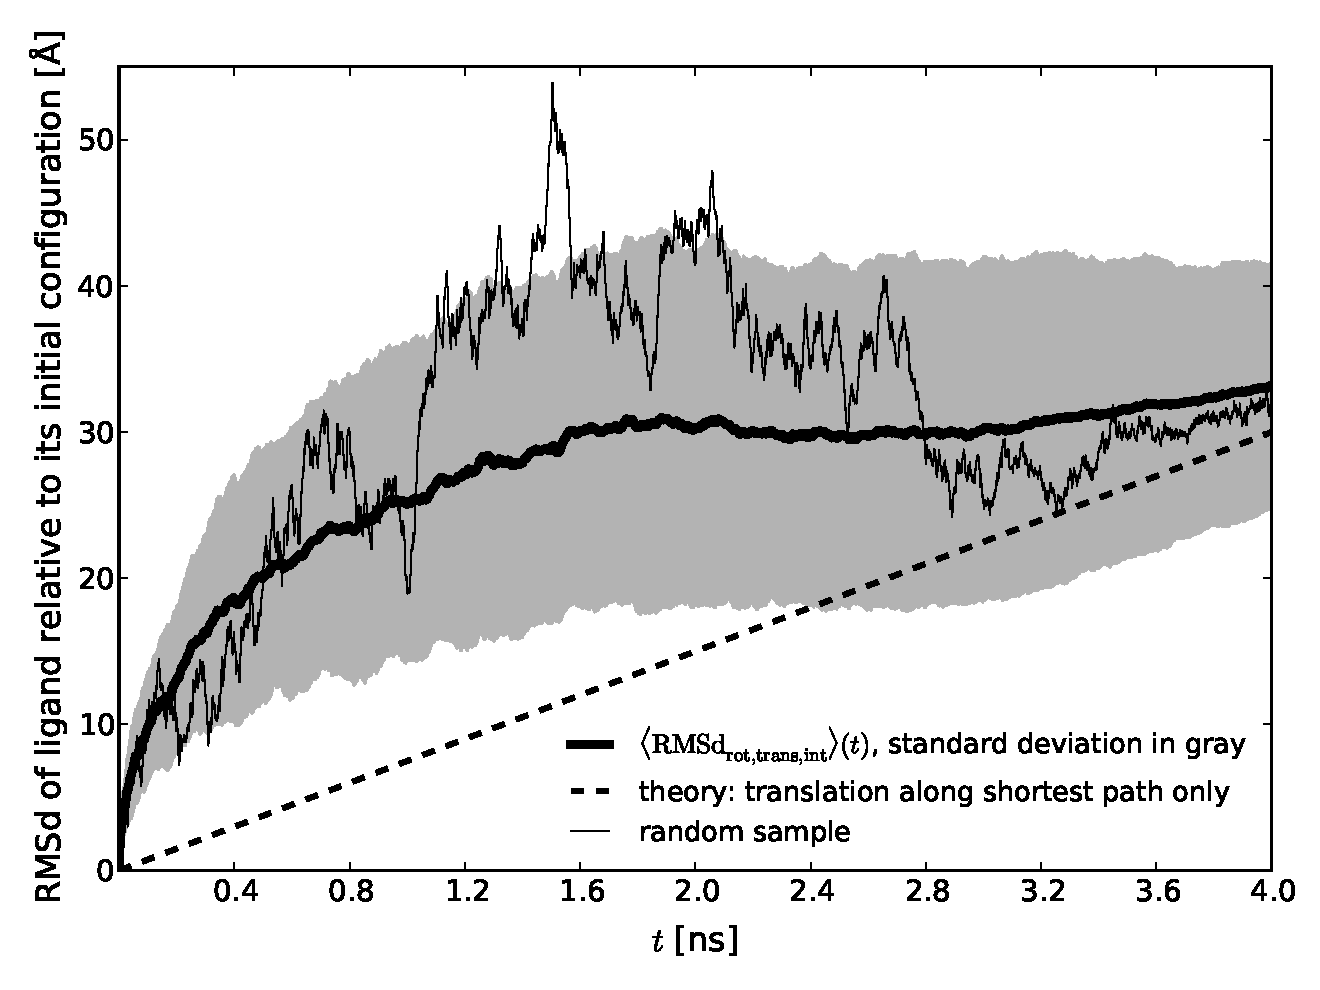
\includegraphics[width=0.9\textwidth]{gfx/dmd/figure_2_freedom_over_time_100samples_avg_stddev_randomone_pub_003.pdf}
\caption[]{
Translational and rotational freedom of a heparin tetramer while approaching
FGF2 during the tMD pulling process with $s=\SI{30}{\angstrom}$ and
\SI{4}{\nano\second}. For each point in time during tMD, the structural difference
between the current and initial ligand configuration was calculated via
classical $RMSd$ and averaged over 100 independent pulling processes. The
variation in ligand movement among different ligand trajectories is visualized
in terms of the standard deviation (grey background).
}
\label{fig:dmd:sampling}
\end{figure}



For the FGF2-HP complex, we compared tMD runs with different pulling velocities
with the goal to find a moderate velocity which still allows significant
translational and rotational ligand movement. In such a case, entirely different
trajectories among tMD repetitions are produced so that Cartesian space sampling
as well as ligand orientation sampling can be enhanced by increasing the number
of tMD repetitions and leaving all other parameters constant. In tMD test runs
with varying duration $T$ but constant ligand displacement length $s$, we
measured the structural difference ($RMSd$) between the current and initial
ligand configuration for each point in time during tMD. Ligand translation,
rotation and internal conformational changes contribute to this time-dependent
structural difference denoted as $RMSd_{\mathrm{rot,trans,int}}(t)$.  The
difference $RMSd_{\mathrm{rot,trans,int}}(t) - ts/T$ describes the extent of
ligand translation and rotation in space compared to the shortest path scenario.

For single test cases with $T=\SI{4}{\nano\second}$ we observed a quickly
fluctuating $RMSd_{\mathrm{rot,trans,int}}(t)$ curve with ligand displacements
from the shortest path between 5 and \SI{40}{\angstrom} $RMSd$. In contrast,
when using $T=\SI{0.5}{\nano\second}$, the displacement varied in the range
between 0 and \SI{10}{\angstrom} $RMSd$. From these data, we could already
conclude that when using $T=\SI{4}{\nano\second}$, the limiting factor for
translational and rotational ligand sampling is the number of tMD repetitions
rather than the pulling velocity. To further quantify the translational and
rotational freedom of the ligand during tMD with $s=\SI{30}{\angstrom}$ and
$T=\SI{4}{\nano\second}$ in detail, we analyzed the deviation of the ligand from
the shortest path for an ensemble of 100 independent tMD runs. To this end, the
structural difference between current and initial ligand configuration was
calculated as described above and then averaged over all 100 independent pulling
processes for each point in time during tMD, leading to $\langle
RMSd_{\mathrm{rot,trans,int}}\rangle(t)$ (\cref{fig:dmd:sampling}). The average
extent of ligand translation and rotation in space turned out to have its
maximum at an $RMSd$ value of about \SI{20}{\angstrom}. The path variation among
ligand trajectories (the standard deviation of the averaged data) is about
$\pm\SI{10}{\angstrom}$ $RMSd$. The data suggest that with
$s=\SI{30}{\angstrom}$ and $T=\SI{4}{\nano\second}$ enough translational and
rotational freedom are provided to the ligand during tMD in order to be
applicable in a local docking method. This also verifies that the extend of
sampling of all ligand DOFs is determined and can be adjusted by the number of
tMD repetitions $N$.

$\langle RMSd_{\mathrm{rot,trans,int}}\rangle$ increases slower after about
$t=\SI{2}{\nano\second}$ (\cref{fig:dmd:sampling}), which is probably caused by
the electrostatic potential of the receptor prevailing against thermally driven
ligand movement. Having this transition included in the $\langle
RMSd_{\mathrm{rot,trans,int}}\rangle(t)$ curve is a good indication for a
properly (long enough) selected initial displacement length $s$. As a general
rule, $s$ should be chosen in a way that no atoms from the initially placed
ligand lie within the non-bonded interaction cut-off range of the receptor.

Due to the type of distance restraint applied, all final tMD states have the
central ligand atom positioned on the surface of the sphere given by the protein
core atom and the final restraint distance $D$. A more robust realization of the
basic DMD concept would not require assigning specific roles to certain points
(core atom and focus point) but implement a dynamic distance restraint between
receptor surface and ligand during the pulling process.

In the current setup, we have compensated for the spherical – and therefore
limited – distribution of tMD final ligand states via careful selection of the
core atom, of $D$, and via a long free MD simulation stage with
$T=\SI{10}{\nano\second}$. This allows for significant ligand refinement
according to the characteristics of the receptor surface as well as for an
exhaustive sampling of the internal DOFs of the ligand. We have quantified the
extent of glycosidic linkage sampling by analyzing the distribution of
glycosidic linkage dihedral values within all free MD simulations of a DMD study
with FGF2 in complex with heparin. Since GLYCAM 06 is known for its proper
description of the glycosidic linkage torsional
potential \cite{kirschner_glycam06:_2008}, we extracted the distribution of
equivalent torsion angles from an independently performed 760 ns MD simulation
of the same heparin molecule free in solution for reference. We compared both
distributions and observed high similarity between them
(\cref{fig:dmd:glycolinkage_sampling}). In particular, the distribution as
observed for the GAG-only simulation is entirely included in the distribution as
observed from the DMD MD simulations where the GAG is in contact with its
protein receptor. In the latter case, some additional conformers seem to be
accessible to the ligand when compared to the GAG-only simulation, which is to
be expected due to its interaction with the receptor. For further
characterization of the sampling, we extracted glycosidic linkage angle values
from 12 PDB entries containing free heparin as well as heparin-protein complexes
(1AXM, 1BFB, 1BFC, 1E0O, 1FQ9, 1G5N, 1GMN, 1HPN, 1QQP, 2AXM, 2HYU, 2HYV) and
observed that this range of experimentally determined angles is included within
the glycosidic torsion angle distribution as sampled by our MD simulations (also
shown in \cref{fig:dmd:glycolinkage_sampling}).


\begin{figure}
\begin{adjustwidth}{-1.5cm}{-1.5cm}
\centering
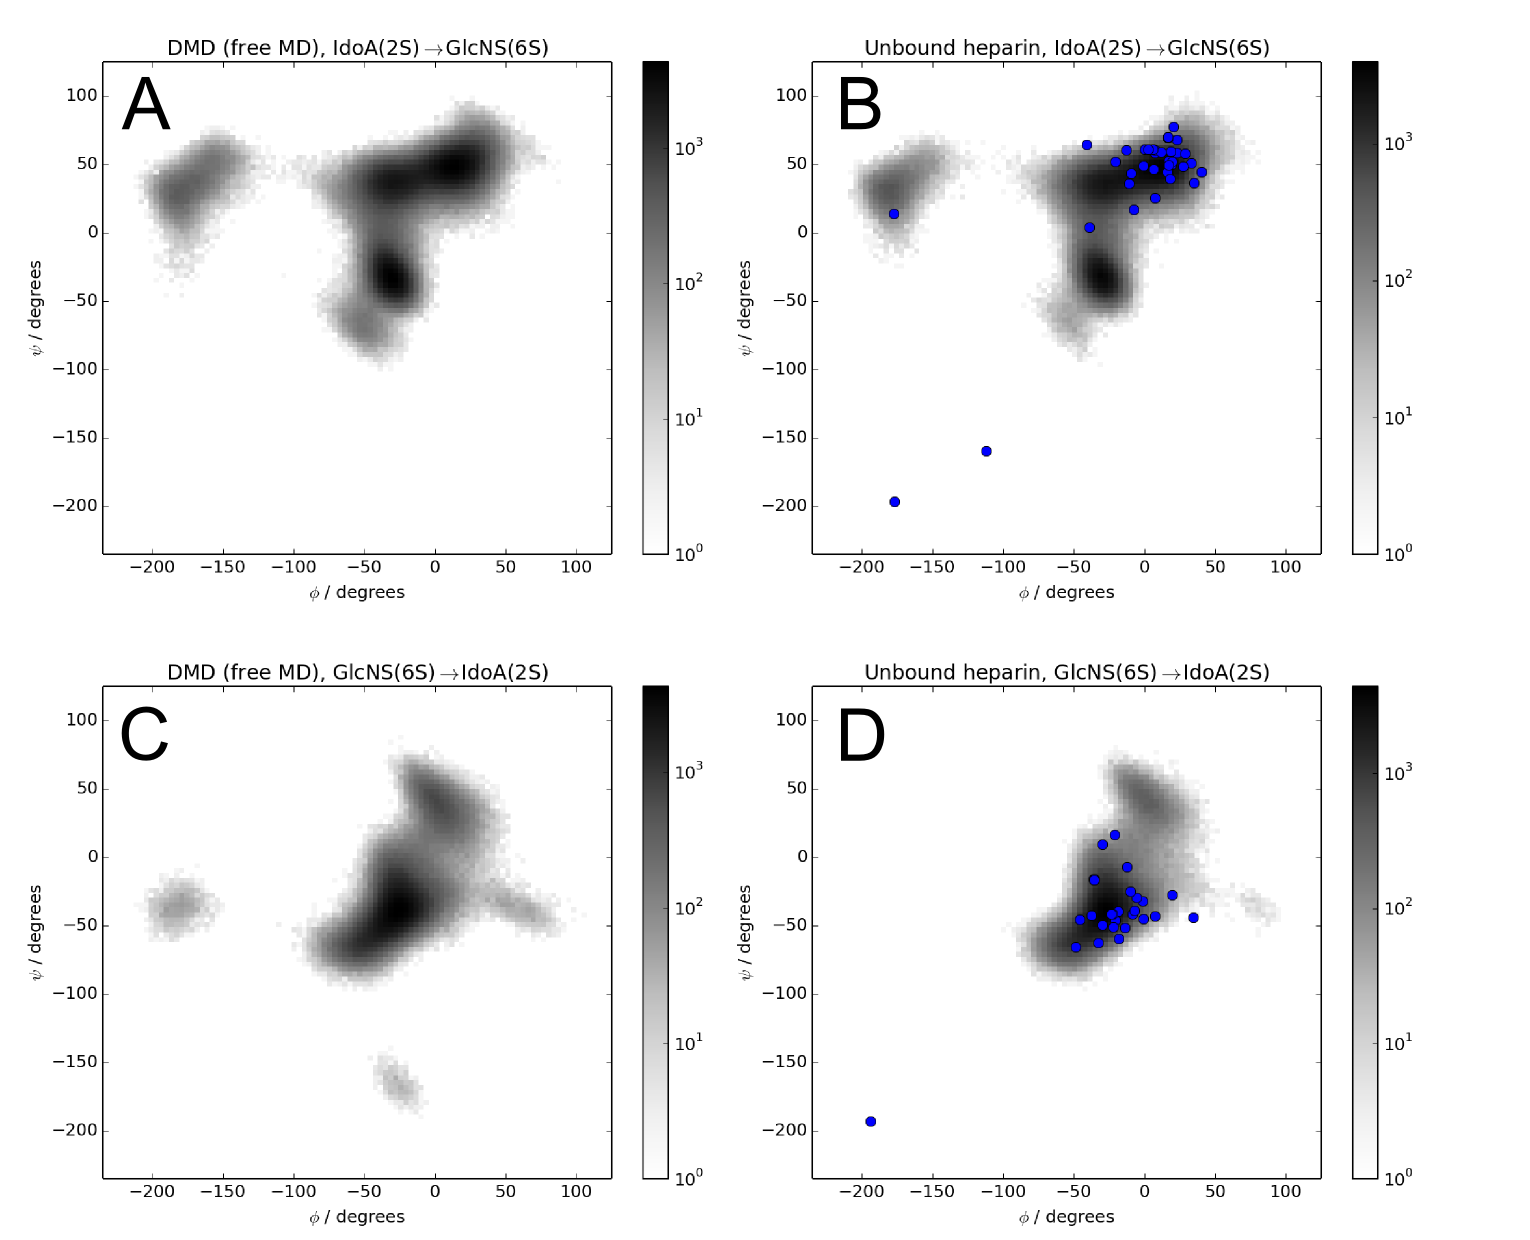
\includegraphics[width=1.3\textwidth]{gfx/dmd/suppl/suppl_glyco_linkage_torsion_maps_03.png}
\caption[]{
Conformational sampling of the glycosidic linkage dihedrals of a free (unbound)
heparin hexasaccharide extracted from 760 ns MD (B, D) compared to the sampling
in all free MD simulations in the DMD study of FGF2-HP (A, C). The torsion
angles are defined as follows: Φ is composed of the atomic chain H1-C1-O4-C4, Ψ
is composed of C1-O4-C4-H4, both in direction from the non-reducing end to the
reducing end of the GAG. All frequency distributions are shown in logarithmic
grey scale. The blue data points in panels B and D additionally show the
distribution of glycosidic linkage dihedral values of heparin as extracted from
the PDB entries 1AXM, 1BFB, 1BFC, 1E0O, 1FQ9, 1G5N, 1GMN, 1HPN, 1QQP, 2AXM,
2HYU, 2HYV (containing unbound as well as bound heparin molecules of different
lengths, the three outliers correspond to terminal sugar monomers).
}
\label{fig:dmd:glycolinkage_sampling}
\end{adjustwidth}
\end{figure}


Most important, we have observed that due to the long free MD stage and a large
number of DMD repetitions, the overall result of a DMD study becomes insensitive
to moderate changes in focus point coordinates as well as in the final tMD
restraint distance $D$.

When visualizing trajectories of tMD and free MD, we repeatedly observed
conceptually different scenarios. In one type of scenario, the ligand ended up
in its native binding pose in the final state of tMD. The conformation of the
ligand then did not undergo significant changes during free MD. In other cases,
the ligand arrived near its anchoring residues on the surface of the receptor
during tMD and then adopted the native binding mode within the free MD
simulation. We also observed the ligand to end up in a false-positive bound
state as well as in an unbound state after tMD or to unbind during free MD.

From these observations we can deduce that if after DMD no agglomeration of
docking solutions stands out, the chosen receptor target region most likely does
not contain a real binding site for the ligand. Furthermore, even if the focus
point of the method is not centered on but only in the vicinity of a real
binding site, the latter most likely stands out during data analysis.

\subsubsection{DMD performance}

\begin{figure}
\centering
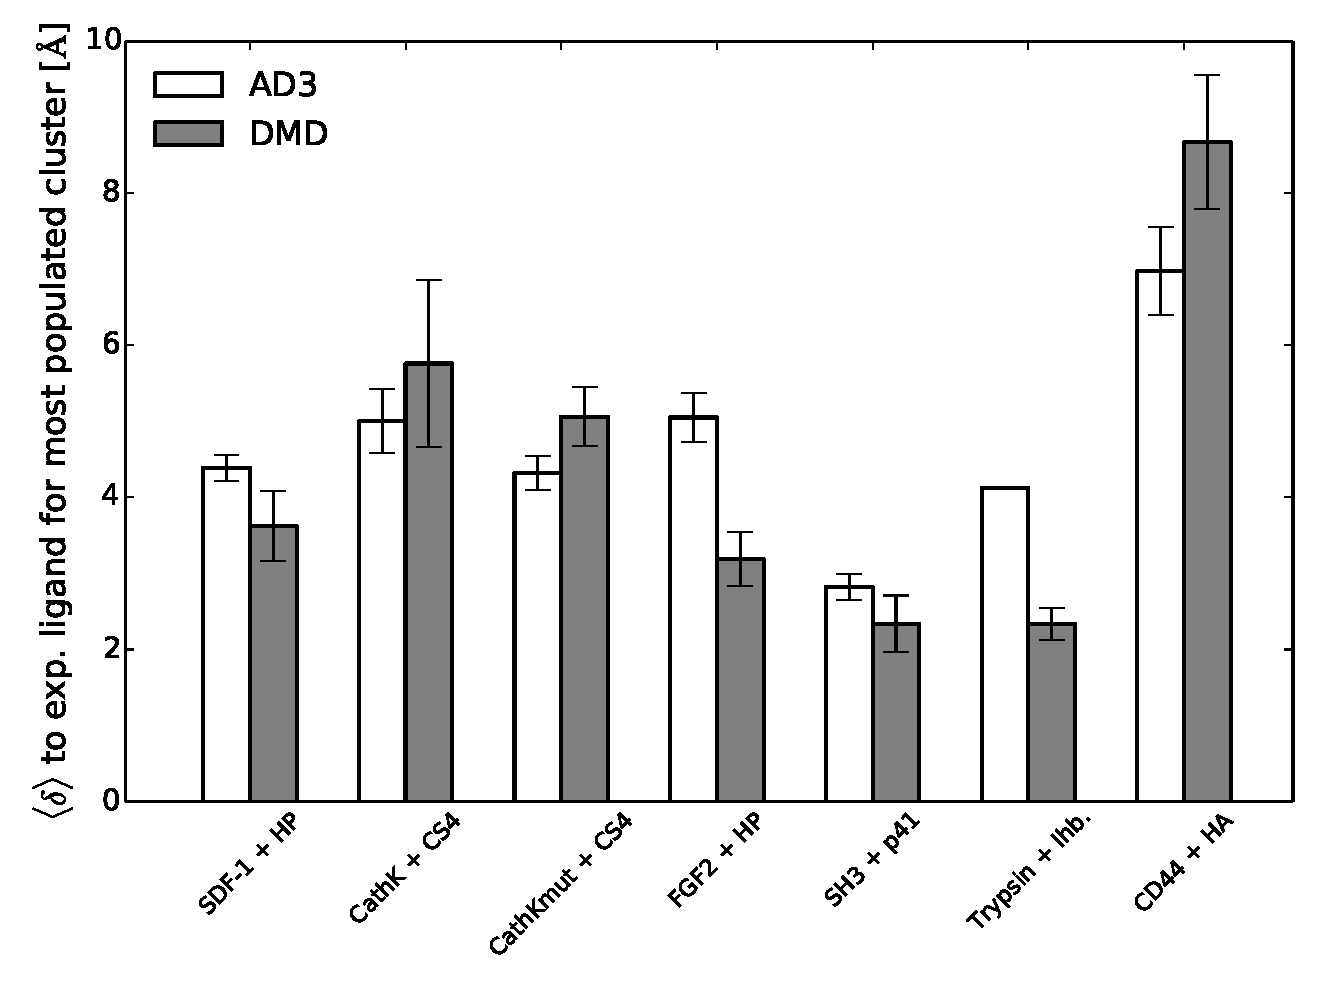
\includegraphics[width=0.9\textwidth]{gfx/dmd/figure_4_clustering_dmd_vs_ad3_plots_pub_004.pdf}
\caption[]{
Mean structural distance $\langle \delta \rangle$ between all members of the
most populated cluster and the experimentally determined ligand for all
investigated complexes with both docking methods. The error bars show the
standard deviation of the mean.
}
\label{fig:dmd:clus_dmd_vs_ad3}
\end{figure}



\begin{table}
\tiny
\centering
\renewcommand{\arraystretch}{1.3}
\begin{tabular}{@{}lcccc@{}}
\multicolumn{5}{c}{\textbf{DMD}} \\
\midrule
Complex & $\epsilon$ / \si{\angstrom} & members & $\delta$ / \si{\angstrom} (mean) &  $\delta$ / \si{\angstrom} (std. dev.) \\
\midrule
CathKmut + CS4 & 3.0 & 6   & 5.1 & 0.4 \\
CathK + CS4    & 3.0 & 4   & 5.8 & 1.1 \\
SDF1 + HE      & 2.2 & 8   & 3.6 & 0.5 \\
CD44 + HA      & 3.2 & 5   & 8.7 & 0.9 \\
SH3 + p41      & 2.6 & 8   & 2.3 & 0.4 \\
FGF + HE       & 2.5 & 6   & 3.2 & 0.4 \\
Trypsin + Ihb. & 1.0 & 9   & 2.3 & 0.2 \\
\midrule
& & & & \\
\multicolumn{5}{c}{\textbf{AD3}} \\
\midrule
Complex & $\epsilon$ / \si{\angstrom} & members & $\delta$ / \si{\angstrom} (mean) &  $\delta$ / \si{\angstrom} (std. dev.) \\
\midrule
CathKmut + CS4  & 2.5 & 6   & 4.3 & 0.2 \\
CathK + CS4     & 2.0 & 9   & 5.0 & 0.4 \\
SDF1 + HE       & 1.2 & 19  & 4.4 & 0.2 \\
CD44 + HA       & 2.5 & 8   & 7.0 & 0.6 \\
SH3 + p41       & 1.8 & 10  & 2.8 & 0.2 \\
FGF + HE        & 1.6 & 10  & 5.1 & 0.3 \\
Trypsin + Ihb.  & 0.1 & 100 & 4.1 & 0.0 \\
\midrule
\end{tabular}
\caption{
Clustering parameters of the most populated cluster for docking solution
ensembles obtained via DMD and AD3. $\epsilon$ is the neighborhood search radius
as used for DBSCAN clustering, $\delta$ measures the structural difference
between two molecules (see Methods).
}
\label{tab:dmd:clustering_parameters}
\end{table}


\vspace{1cm}
\textbf{Spatial distribution of docking solutions.}
We compared the performance of DMD with the performance of the well-established
AD3 docking approach, which was used for other molecular systems including GAGs.
We applied DMD and AD3 to all TDS complexes and analyzed the spatial
distribution of docking results via clustering
(see \cref{tab:dmd:clustering_parameters}). For each
complex, we compared the mean structural distance $\langle \delta \rangle$
between the experimentally determined ligand position and all members of the
most populated cluster (\cref{fig:dmd:clus_dmd_vs_ad3}). In terms of the
capability to produce solutions structurally close to the experimentally
determined ones, both docking methods perform comparably well. However,
interesting differences are observable. AD3 generally yields smaller spatial
scattering of solutions as given by the standard deviation of data points in
\cref{fig:dmd:clus_dmd_vs_ad3}. This can be attributed to the static treatment
of the receptor by AD3. Notably, we can generally conclude that DMD performed
better than AD3 for the complexes with strongest electrostatic attraction,
namely SDF-1-HP and FGF2-HP. For the FGF2-HP complex, the most populated cluster
from DMD reproduces the experimentally determined HP binding pose, while the
most populated cluster from AD3 docking only partially overlaps with this pose
(\cref{fig:dmd:fgf2zoom}a). In fact, DMD was able to identify the
\enquote{higher affinity} binding site for heparin (as denoted in the original
publication of the FGF2-HP crystal structure), while AD3 identified the
\enquote{lower affinity} site, which becomes occupied upon heparin
hexasaccharide binding \cite{faham_heparin_1996}. In addition, DMD was able to
properly predict the positioning of the two sulfate groups making specific high-
affinity contact to FGF2 (\cref{fig:dmd:fgf2zoom}b). These two sulfate groups
form seven of the nine polar contacts between FGF2 and HP and therefore are
important anchoring groups for the molecular recognition
\cite{faham_heparin_1996}. The fact that DMD was able to reproduce this key
feature as opposed to AD3 most probably reflects the crucial role of receptor
flexibility considered in the docking simulation.

\begin{figure}
\centering
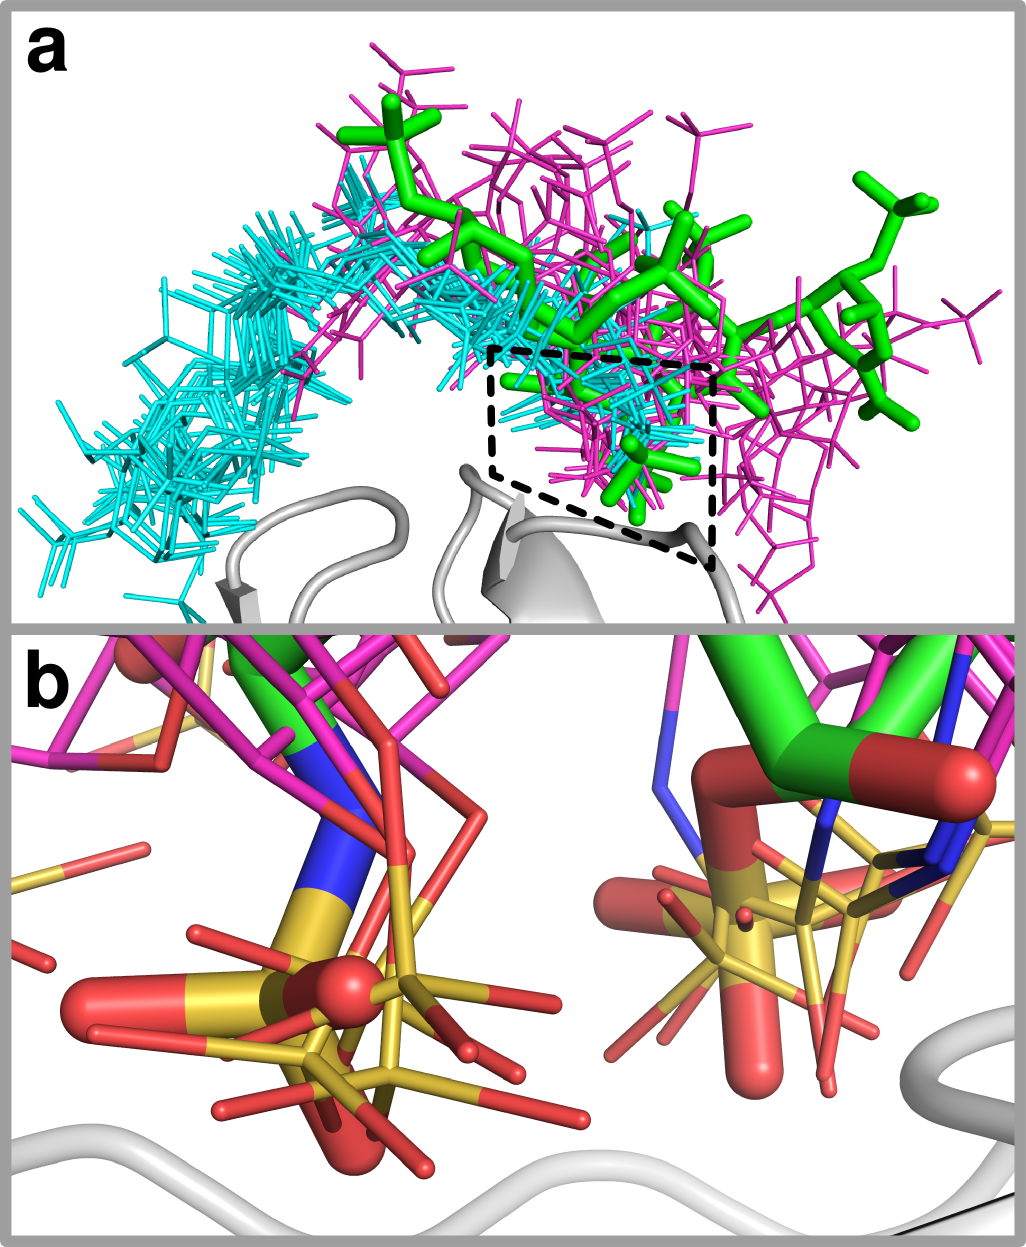
\includegraphics[width=0.9\textwidth]{gfx/dmd/fgf2_topclusters_dmd_vs_ad3_receptorribbon_normal_and_zoom_jcc_004.png}
\caption[]{
Docking results from DMD and AD3 for FGF2 (grey cartoon representation) and HP.
\textbf{a}: ligand from crystal structure in green sticks. Most populated
cluster of DMD solutions in magenta. Most populated cluster of AD3 solutions in
cyan. \textbf{b}: zoom on two sulfate groups making specific high-affinity
contact to FGF2 \cite{faham_heparin_1996} (as marked in \textbf{a} via dashed
line). Ligand from crystal structure with C atoms in green (thick sticks). Most
populated DMD cluster with C atoms in magenta (thin sticks).
}
\label{fig:dmd:fgf2zoom}
\end{figure}


In order to assess the ability of DMD to predict consistent binding poses for
GAGs differing in length, we carried out additional DMD studies for SDF-1 as
well as FGF2. Eventually, both systems were investigated with independent DMD
studies for each of di-, tetra- and hexasaccharides of heparin. For FGF2-HP, the
two sulfate groups making specific contact to FGF2 were identified when docking
both an HP tetrasaccharide and an HP hexasaccharide. These observations support
the assumption that GAG fragments differing in length share key interactions
with the protein. When docking an HP disaccharide, those key interactions were
not identified, suggesting that the disaccharide is not long enough to maintain
specificity. Nevertheless, for the SDF-1-HP and FGF2-HP systems, we observe that
all obtained poses overlap regardless of the GAG length
(\cref{fig:dmd:fgf2_hp_246,fig:dmd:sdf1_hp_246}).  A direct visual comparison
between the crystal structure of FGF2 with a heparin
hexasaccharide \cite{faham_heparin_1996} and the corresponding DMD result can
be seen in \cref{fig:dmd:fgf2_hp_246}.


\begin{figure}
\centering
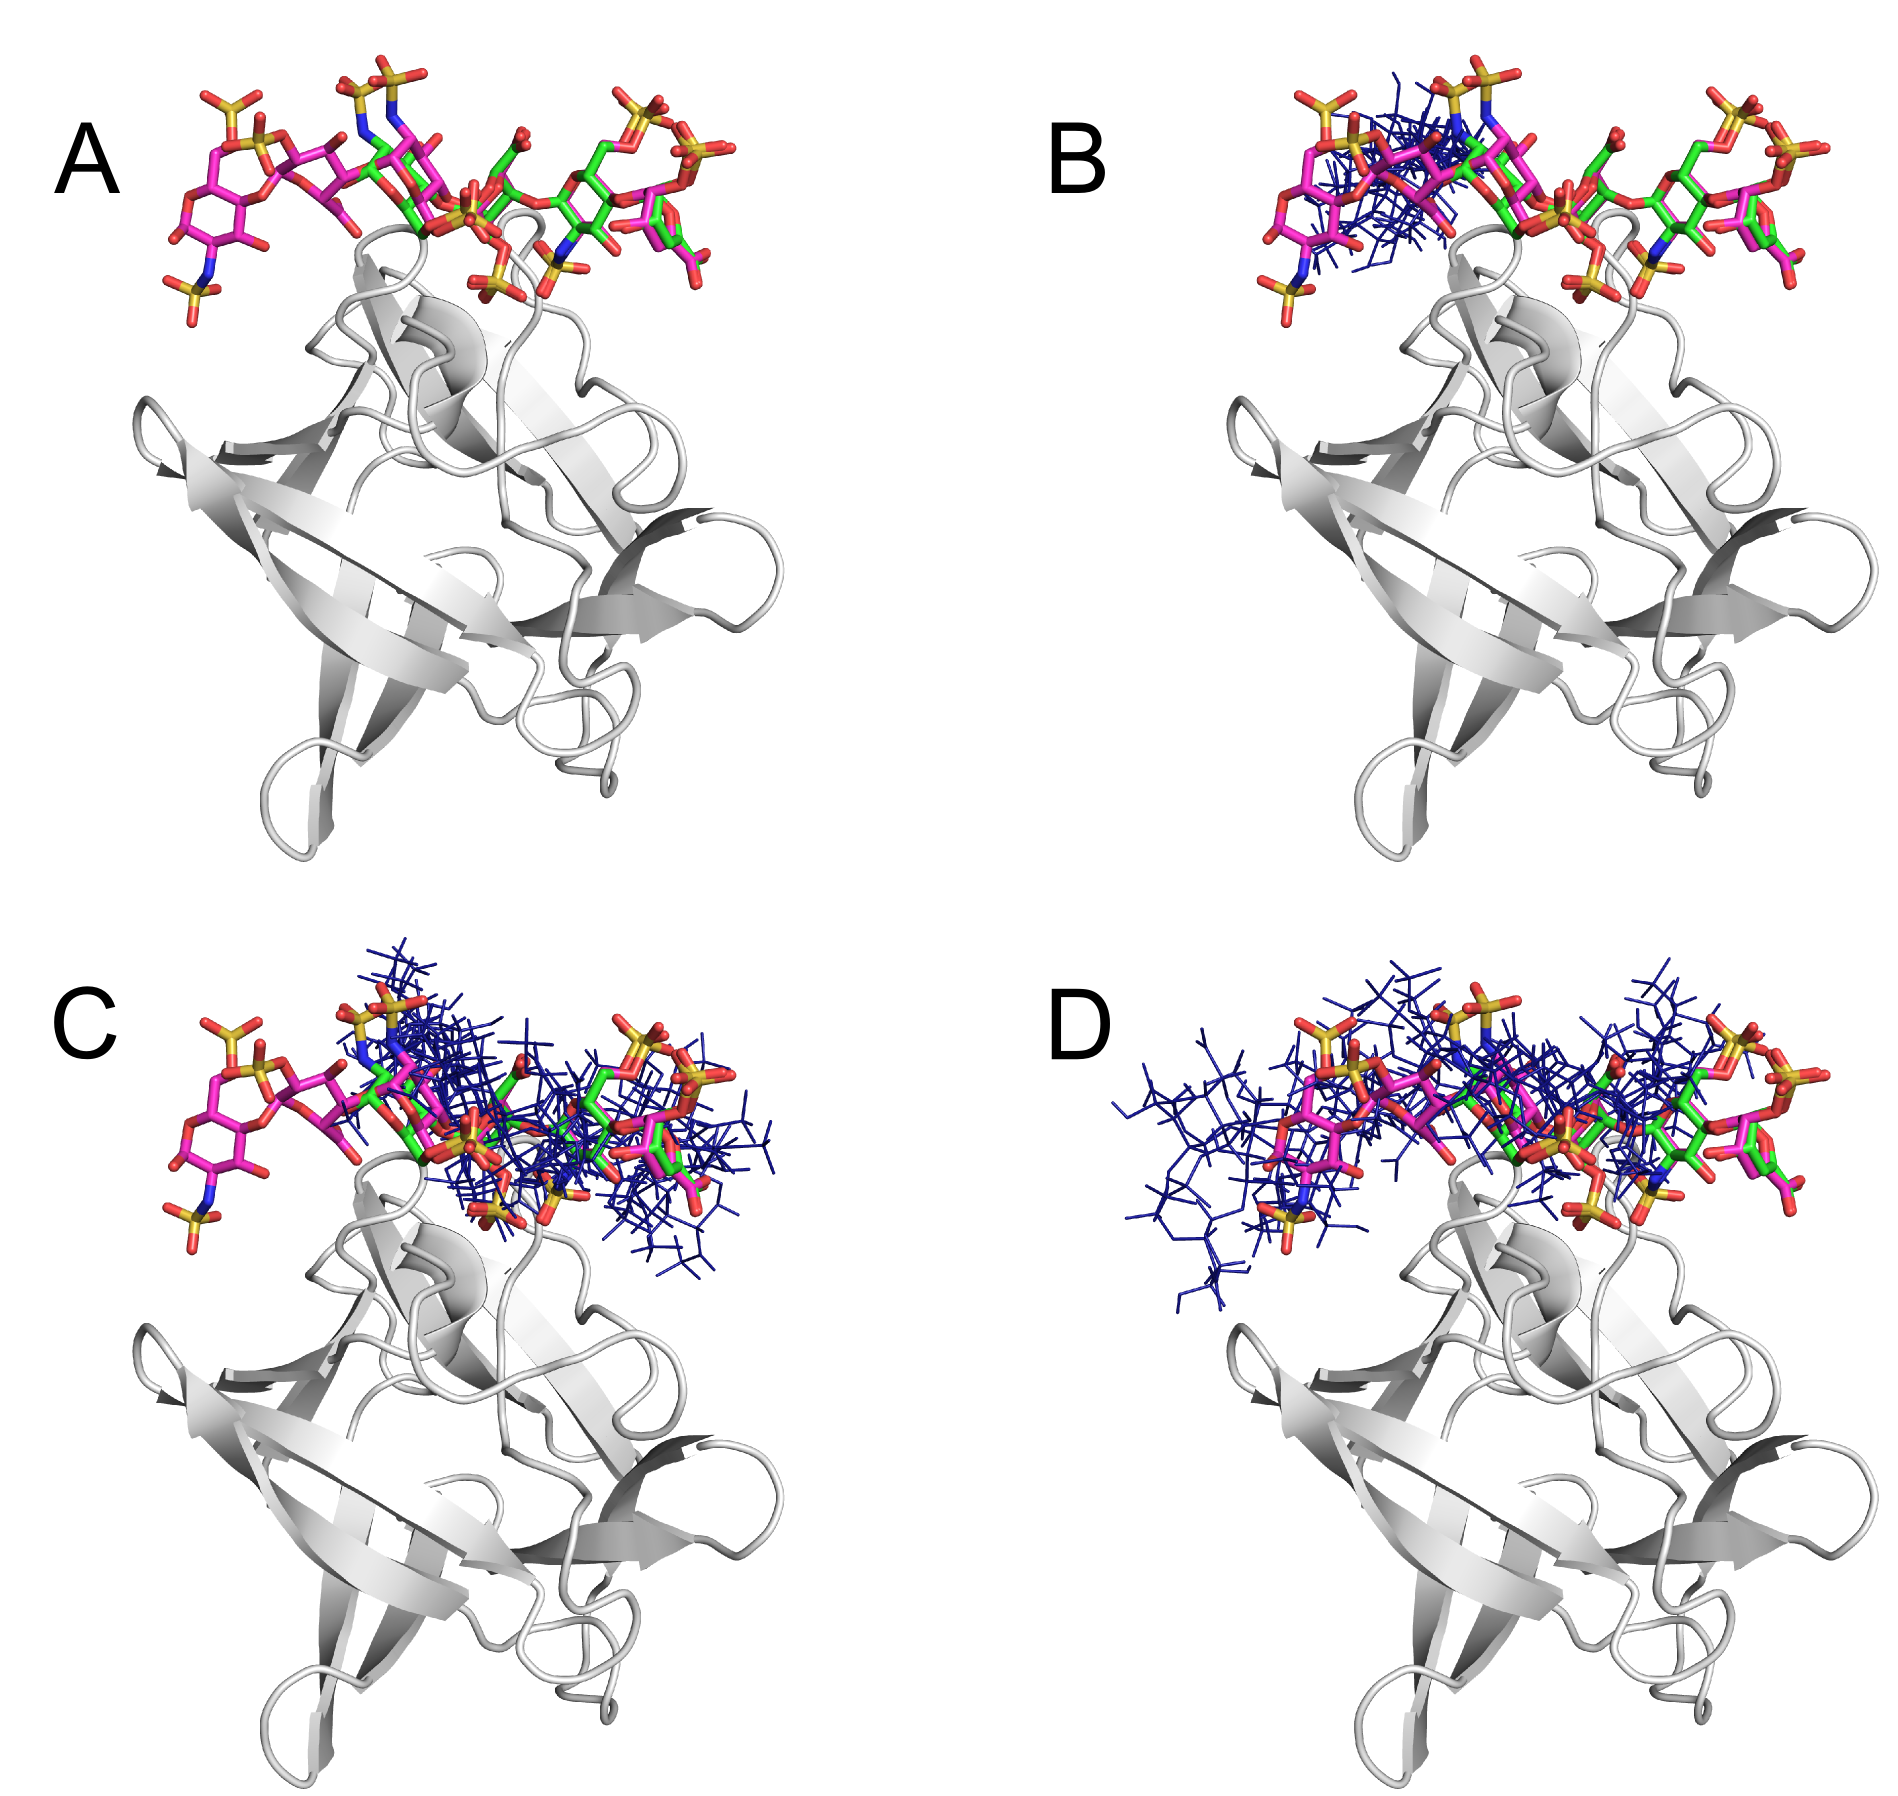
\includegraphics[width=0.9\textwidth]{gfx/dmd/suppl/suppl_fgf2_dmd_he-2-4-6_02.png}
\caption[]{
DMD results for FGF2 in complex with a heparin di-, tetra- and hexasaccharide.
In magenta and green sticks, the heparin hexamer and tetramer poses as
determined experimentally are shown (PDB IDs 1BFB, 1BFC), respectively. The most
populated clusters for di-, tetra- and hexasaccharide docking solutions are
shown in B, C, D, respectively, as blue sticks. The protein is shown in grey
cartoon.
}
\label{fig:dmd:fgf2_hp_246}
\end{figure}


\begin{figure}
\centering
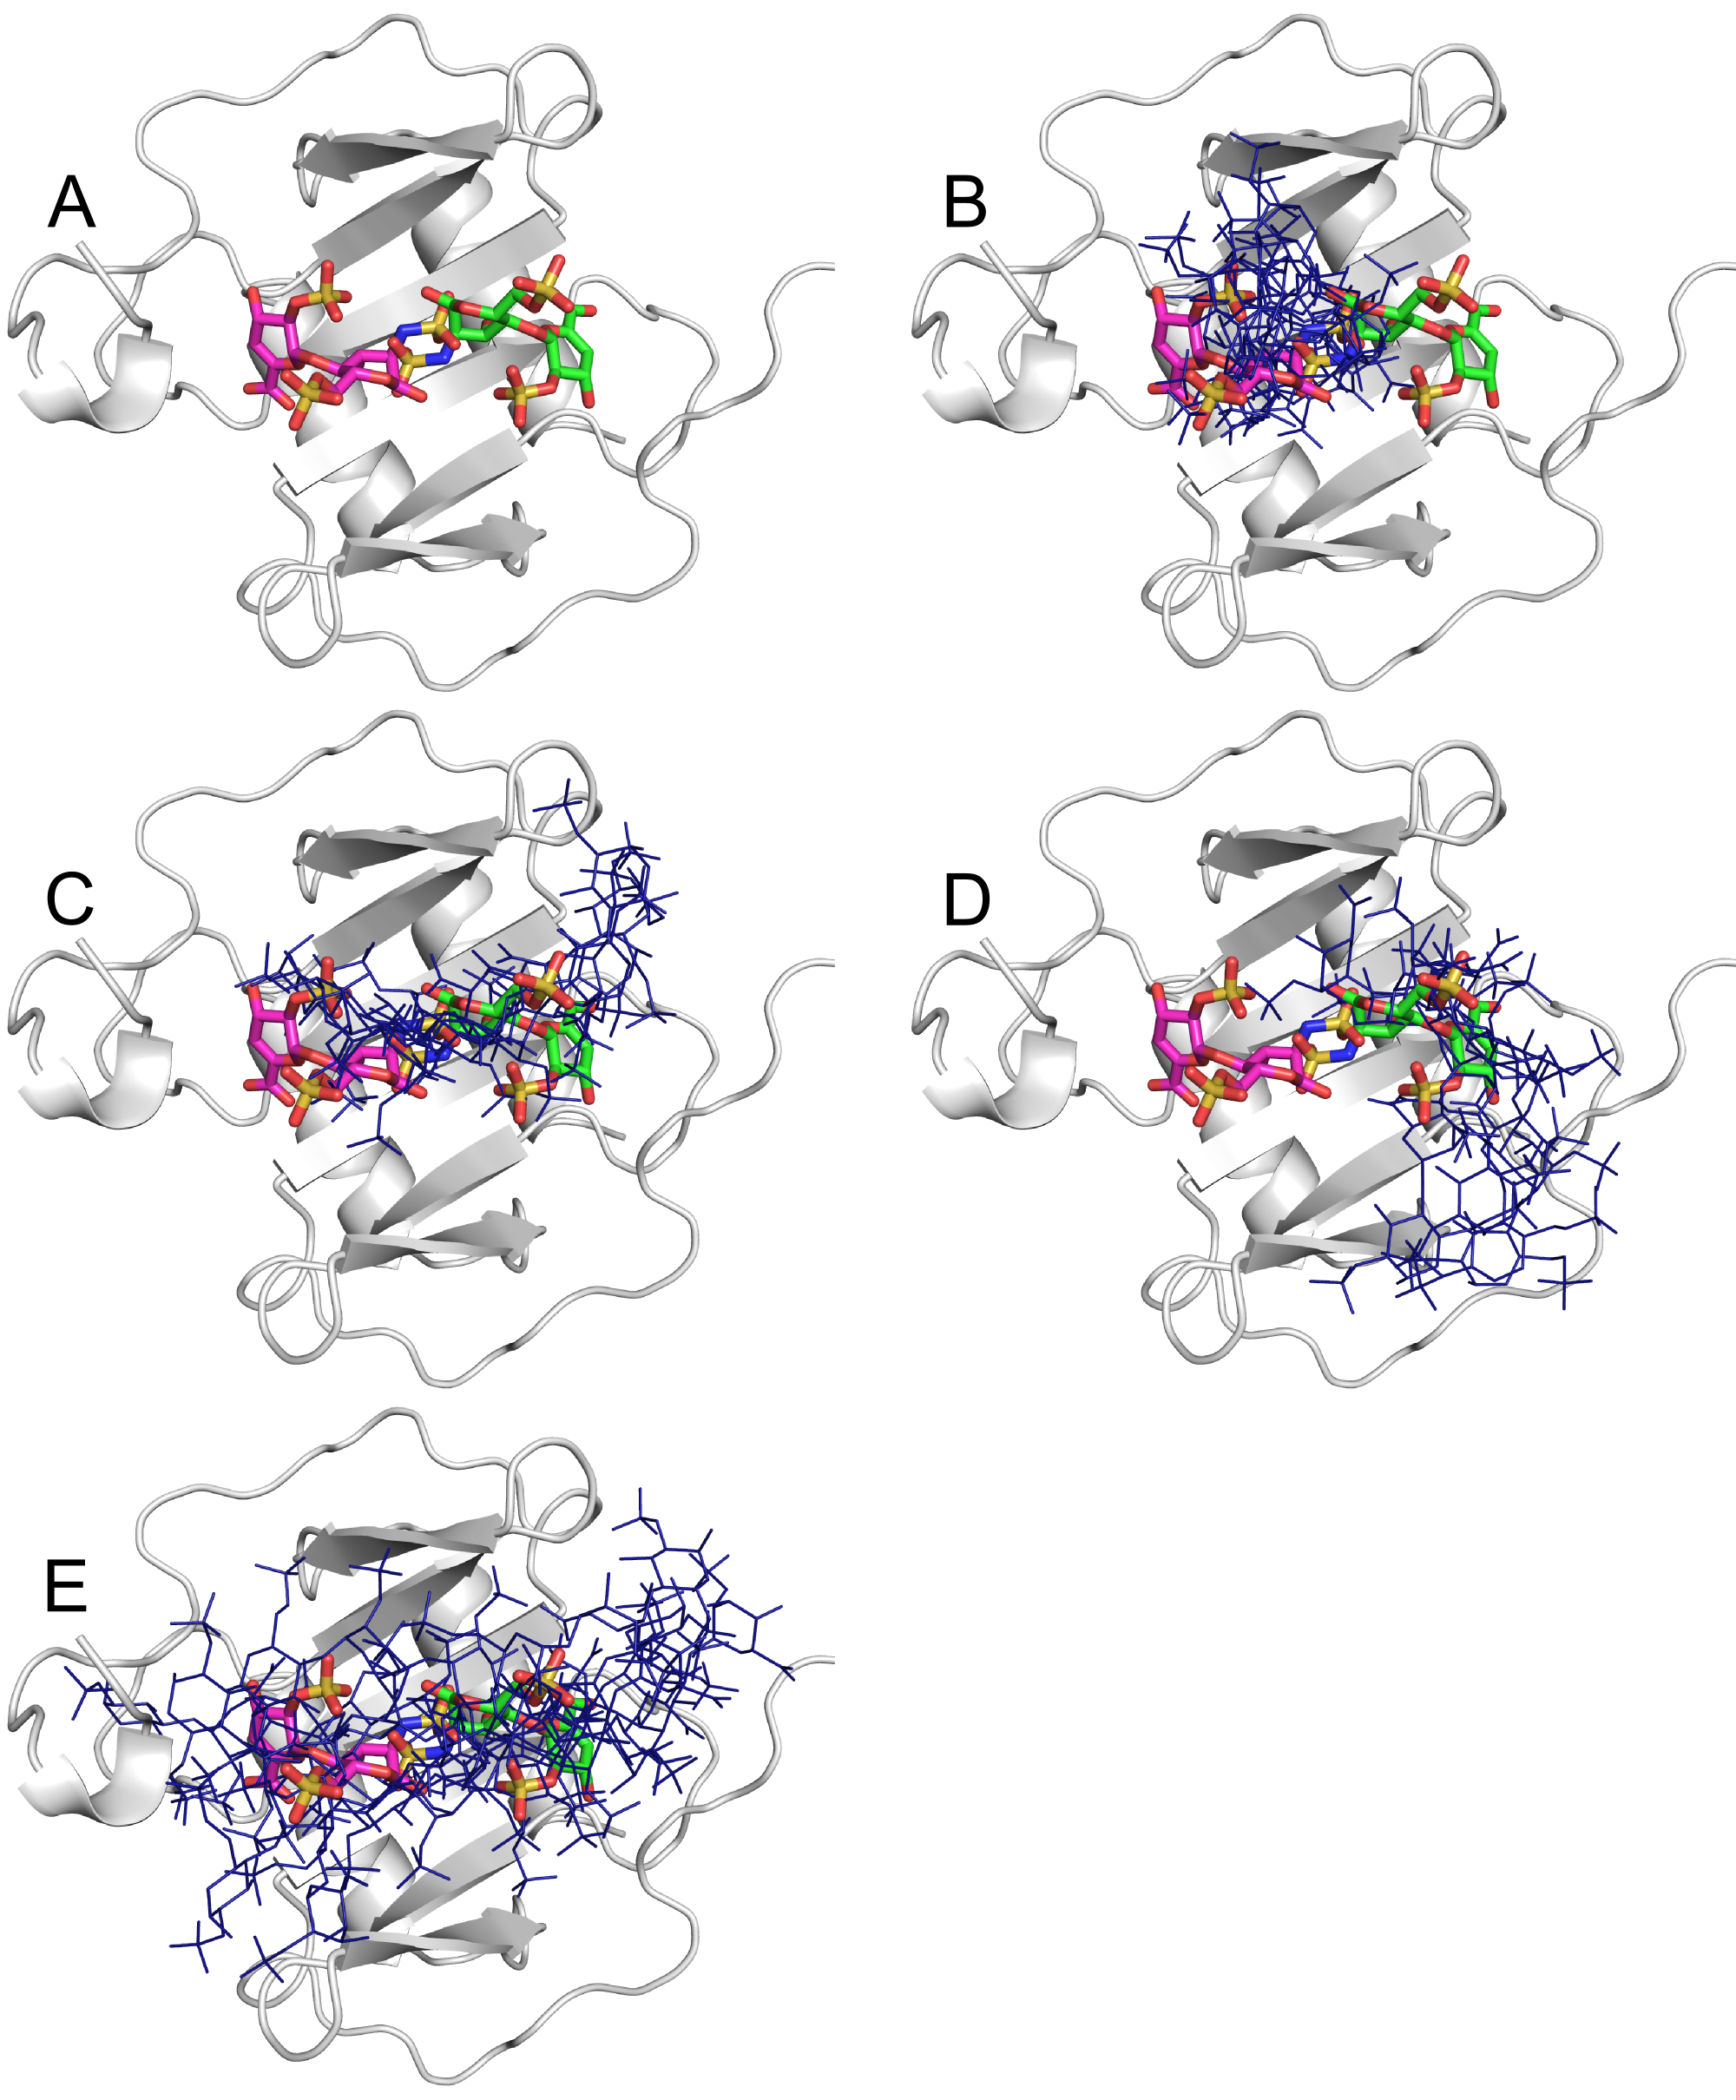
\includegraphics[width=0.9\textwidth]{gfx/dmd/suppl/suppl_sdf1_dmd_he-2-4-6.png}
\caption[]{
DMD results for SDF-1 in complex with a heparin di-, tetra- and hexasaccharide.
In magenta sticks, the heparin dimer pose as determined experimentally is shown
(PDB ID 2NWG). For clarity, we show its symmetric counterpart (180 degree
rotation about the 2-fold axis of the SDF-1 dimer) in green sticks. The most
populated clusters for di-, tetra- and hexasaccharide docking solutions are
shown in B, C \& D, E, respectively, as blue sticks. The protein is shown in
grey cartoon.
}
\label{fig:dmd:sdf1_hp_246}
\end{figure}


As has been conceptually described for the FGF2-HP complex, also regarding the
SH3-p41 and Trypsin-inhibitor complexes, DMD provided solutions closer to the
experimentally determined ones while displaying a more diverse scattering of
docking solutions than AD3.

For CD44 in complex with the HA heptamer, both docking methods were only
partially able to reproduce the experimentally determined ligand pose. Weak net
electrostatic repulsion between receptor and ligand seemingly imposes a major
challenge for both docking methods. AD3 and DMD solutions, however, are
spatially consistent (data not shown).

Both docking methods had difficulties reproducing the experimentally determined
binding poses of CathK and CathKmut in complex with CS4. In case of CathK-CS4,
the crystal structure contains a single high molecular weight polymeric CS4
molecule interacting with multiple copies of the same protein
\cite{catK_cs4_crystal_structure_2008}. Within the CathKmut-CS4 crystal, each
GAG hexamer tightly interacts with two CathKmut proteins
\cite{catKmut_cs4_crystal_2011}. Under these conditions, it is to be expected
that considering only a short GAG and a single protein in the docking experiment
is not sufficient to allow for an accurate reproduction of the experimentally
determined structures.

The presented structural difference comparison between DMD and AD3-based docking
solutions and the corresponding experimentally determined ligand coordinates is
subject to a systematic error. Structural relaxation prior to docking with AD3
changed the receptor side chains in the binding region by a heavy atom $RMSd$ of
\SI{1.0 +- 0.4}{\angstrom} (mean value and standard deviation derived from all
TDS complexes) when compared to the experimentally determined receptor
structure. The solutions from DMD display a mean binding region alteration of
\SI{2.3 +- 0.6}{\angstrom} (corresponding raw data is shown in
\cref{tab:dmd:binding_site_rmsd}). The larger the binding site alteration, the
more error-prone the comparison between docked solution and experimentally
determined ligand becomes. Under the assumption that this error systematically
increases the structural difference, DMD might have performed better compared to
AD3 than shown in Figure 4.


% http://www.inf.ethz.ch/personal/markusp/teaching/guides/guide-tables.pdf
\begin{table}
\tiny
\centering
\renewcommand{\arraystretch}{1.3}
\begin{tabular}{@{}lcccc@{}}
\toprule
& \multicolumn{2}{c}{\textbf{DMD (after free MD)}} & \multicolumn{2}{c}{\textbf{AD3}} \\
Complex & Entire receptor & Binding site &  Entire receptor & Binding site \\
\midrule
SDF-1 + HP & 3.6 $\pm$ 0.5 & 2.3 $\pm$ 0.5 &  0.4 & 0.2 \\
CathK + CS4 & 1.8 $\pm$ 0.2 & 2.0 $\pm$ 0.3 & 1.1 & 1.2 \\
CathKmut + CS4 & 1.8 $\pm$ 0.2 & 1.9 $\pm$ 0.4 & 1.1 & 1.4 \\
FGF2 + HP & 3.4 $\pm$ 0.1 & 3.6 $\pm$ 0.1 & 1.3 & 1.1 \\
SH3 + p41 & 2.2 $\pm$ 0.2&  2.4 $\pm$ 0.4 &  1.3 & 1.4 \\
Trypsin + Ihb. & 1.6 $\pm$ 0.1 & 1.5 $\pm$ 0.4 & 0.9 & 0.7 \\
CD44 + HA & 2.2 $\pm$ 0.3 & 2.5 $\pm$ 0.5 & 0.9 & 0.7 \\
\bottomrule
\end{tabular}
\caption{
Heavy atom RMSd between experimentally determined structure of the receptors and
the receptor structures corresponding to the docking solutions. Differences were
obtained for \textit{i} the entire receptor and \textit{ii)} the binding site
only as determined by the MOE \enquote{pocket} feature. In case of DMD, mean
distances $\pm$ standard deviation were obtained from 100 independent free MD
runs per complex. Numbers are given in ångströms.
}
\label{tab:dmd:binding_site_rmsd}
\end{table}

\vspace{1cm}
\textbf{Identification of anchoring residues in the ligand binding
region.} The prediction of receptor residues important for ligand binding is of
particular practical value. While AD3 does not provide energetic data on the
single-residue level, DMD allows for a single-residue energy decomposition
(SRED) based on time-averaged free MD interaction energy data.

For each TDS complex, we merged SRED data from the entire ensemble of DMD runs
and extracted the set of anchoring residues, which are at most ten of the
receptor residues contributing most (positively) to ligand binding. We also
determined a reference set of anchoring residues from MD simulations of the
experimentally determined structures. For each TDS complex, we then identified
the intersection of both sets (\cref{tab:dmd:anchoring_receptor_redidues}).


\begin{table}
\tiny
  \centering
  \smallskip
  \begin{threeparttable}
    {\renewcommand{\arraystretch}{1.3}%
      \begin{tabular}{lcccr}
      \hline
      \textbf{Complex} & \specialcell{\textbf{Number of correctly} \\ \textbf{predicted residues}\tnote{a}} &
      \specialcell{\textbf{Number of} \\ \textbf{charged residues}} &
      \specialcell{\textbf{Number of polar} \\ \textbf{uncharged residues}} & $r$\tnote{b} \\ \hline
      SDF-1 + HP & 7 of 10 & 7 & 0 & 0.52 \\
      CathK + CS4 & 6 of 10 & 4 & 2 & -0.21 \\
      CathKmut + CS4 & 6 of 10 & 4 & 1 & -0.12 \\
      FGF2 + HP & 9 of 10 & 6 & 2 & 0.84 \\
      SH3 + p41 & 2 of 5 & 0 & 0 & -- \\
      Trypsin + Ihb. & 5 of 10 & 2 & 2 & 0.73 \\
      CD44 + HA & 1 of 7 & 1 & 0 & -- \\ \hline
      \end{tabular}
    }
    \begin{tablenotes}
      \item[a] Number of predicted receptor anchoring residues having a match in
      the reference set (as obtained from SRED via MD of the experimentally determined structures).
      \item[b] Spearman's rank correlation $r$ between the SRED-energies of both residue sets
      (calculated only if five or more residues match).
    \end{tablenotes}
  \end{threeparttable}
\caption{Predictive power of DMD for the identification of receptor anchoring residues.}
\label{tab:dmd:anchoring_receptor_redidues}
\end{table}


For Trypsin in complex with its inhibitor, half of the anchoring residues in the
crystal structure were correctly found. For SDF-1-HP, CathK-CS4, and
CathKmut-CS4 more than half of the anchoring residues were identified by SRED.
Furthermore, for the FGF2-HP complex, nine of ten anchoring residues were
predicted properly.

In order to evaluate the capability of DMD to rank the receptor anchoring
residues according to their importance for ligand binding, we calculated
Spearman's rank correlation between the SRED-energies of residues in both, the
reference and comparison sets (\cref{tab:dmd:anchoring_receptor_redidues}). For
three of those five complexes with at least five predicted anchoring residues,
the DMD ranking turned out to reproduce the reference ranking quite well
(SDF-1-HP, FGF2-HP, Trypsin-Ihb). For the CathK-CS4 and CathKmut-CS4 complexes
the anchoring residue ranking was not reproduced.

\begin{figure}
\centering
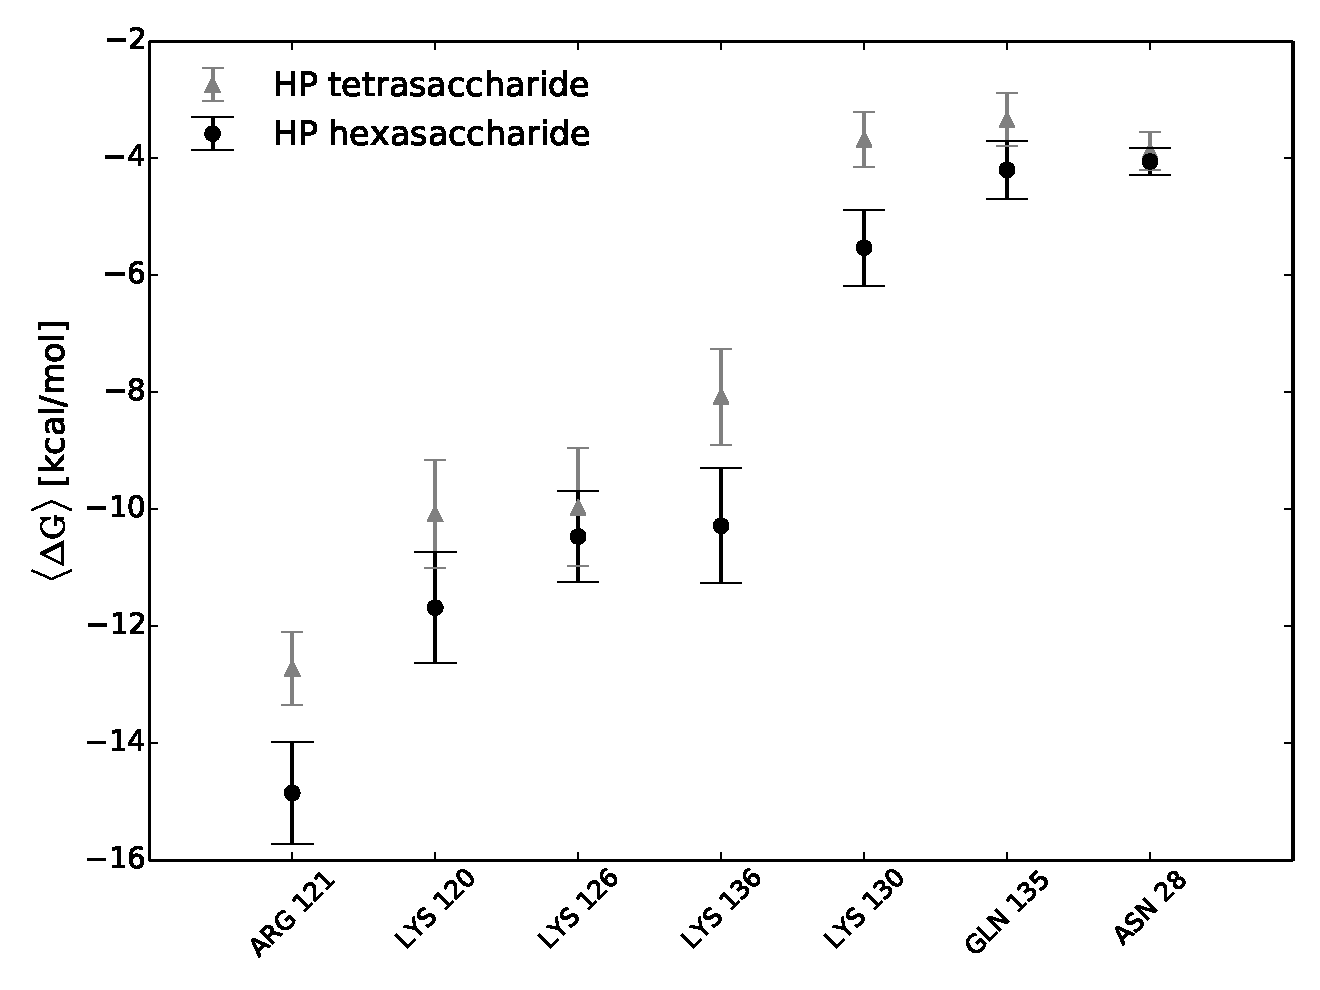
\includegraphics[width=0.9\textwidth]{gfx/dmd/figure_6_receptor_top7_residues_of_top_40percent_dmd_runs.pdf}
\caption[]{
FGF2 amino acid residues identified by DMD as having the greatest impact on
FGF2-HP binding. Results are shown for both heparin tetra- and hexasaccharide
ligands as retrieved from two independent DMD studies. For each residue, an
average energy ($\pm$ standard error of the mean) for the interaction with the
ligand is shown as obtained from 40 independent free MD simulations.
}
\label{fig:dmd:sred_fgf2}
\end{figure}

Based on the obtained results, we can conclude that for systems dominated by
electrostatic attraction such as protein-GAG systems, DMD is capable of
correctly identifying those amino acid residues responsible for forming key
interactions with the ligand. Regarding the FGF2-HP system, we found that both
heparin tetra- and hexasaccharide docking via DMD enabled us to consistently
identify the same chemical groups in the GAG molecule being key for binding.
Moreover, using SRED data, we were able to demonstrate that the identified key
amino acid residues as well as their energy ranking are identical when comparing
heparin tetra- and hexasaccharide docking performed in independent DMD studies
(see \cref{fig:dmd:sred_fgf2}). This observation supports the idea that,
regardless of their length, GAG fragments preserve their key interactions with
certain protein amino acid residues. The set of FGF2 key amino acid residues as
identified by SRED contains all residues that were crystallographically
characterized as most important for binding (R121, K126, N28,
Q135) \cite{faham_heparin_1996}. Based on our data we can additionally state
that also residue K120 is of major importance, since it acts as hydrogen bond
donor in a similar way as K126 does. The latter observation is in agreement with
previous calorimetry studies pointing out the importance of K120 in the FGF2-HP
system \cite{thompson_1994_fgf2_heparin}. These findings motivate the
application of DMD to systems in which a detailed and appropriate description of
GAG recognition is required.



\subsubsection{Electrostatic potential analysis in the context of DMD}

Our electrostatic potential evaluation procedure as discussed in
\cref{chapter:bspred} unambiguously identifies the GAG binding sites as
determined experimentally for SDF-1-HP as well as the FGF2-HP systems. Analysis
of CD44's Coulomb potential revealed that the net electrostatic interaction
between CD44 and HA is either insignificant or even slightly repulsive. These
findings seem to be directly correlated to the success of DMD in terms of
reproducing the natural ligand binding mode, which can be described as failure
in case of the CD44-HA system. We observe that electrostatic potential analysis
provides a clear idea whether GAG-binding to a given receptor is mainly driven
by Coulomb interaction. If a protein is known to bind GAGs, and the
electrostatic potential topology is as unambiguous as in case of SDF-1 or FGF2,
a GAG binding site prediction based on the procedure presented in
\cref{chapter:bspred} is reliable and can be used for planning a DMD study for a
given system. Visualization of the electrostatic potential can in any case be
helpful to \textit{a priori} exclude regions of the receptor surface when
repulsive to negatively charged ligands. Especially, knowledge about the
electrostatic potential distribution in space can be used to choose a reasonable
ligand \enquote{entry lane} orientation for the tMD pulling process.


\subsubsection{General discussion}

In summary, our data suggest that DMD is able to yield docking results of high
significance, especially in case of receptor-ligand systems dominated by
attractive electrostatic interaction. This success is well-grounded by the
concept that the ligand --- while slowly approaching the receptor surface ---
performs extensive conformational sampling and, at the same time, responds to
the long-range Coulomb potential of the receptor. During the pulling process,
the Coulomb potential significantly contributes to steering the entirely
flexible and charged ligand towards its binding site and to let it finally adopt
its binding pose in an explicit solvent environment. The subsequent free MD step
allows for an unbiased mutual adjustment of receptor residues and ligand.

DMD is a local docking method focused towards a certain region on the receptor
surface. When selecting focus point, core atom, and target distance $D$, one
needs to ensure that after the pulling process, the ligand is able to establish
short-range interactions within the receptor binding region but is not forced
into clashes with the receptor. In our study, we selected the focus point based
on the experimentally determined ligand position and could therefore easily
determine the required MD target distance values
(\cref{tab:dmd:tds_target_distances}). In practice, when the structure of the
bound ligand is unknown, the focus point has to be defined based on the residues
comprising the putative binding region and based on binding mode assumptions,
for instance generated by classical docking methods or by manual docking .

\begin{table}
\scriptsize
\centering
\renewcommand{\arraystretch}{1.3}
\begin{tabular}{@{}lr@{}}
\toprule
Complex & $D$ / \si{\angstrom} \\
\midrule
SDF-1 + HP & 10.6 \\
CathK + CS4 & 19.2 \\
CathKmut + CS4 & 20.9 \\
FGF2 + HP & 25.0 \\
SH3 + p41 & 7.7 \\
Trypsin + Ihb. & 12.1 \\
CD44 + HA & 15.3 \\
\bottomrule
\end{tabular}
\caption{
Target distance $D$ as applied during the tMD simulations for any given TDS complex.
}
\label{tab:dmd:tds_target_distances}
\end{table}


One of the main concepts of DMD is that pulling process and subsequent free MD
are repeated many times in independent simulations. This allows for the creation
and evaluation of an ensemble of docking solutions rather than the
interpretation of single trajectories. In this ensemble, the energetically more
favorable states are the more likely ones. Spatial clustering of this docking
solution ensemble identifies those docking solutions that appeared with highest
probability and, therefore, lowest energy. With respect to the identification of
anchoring residues in the receptor and their energetical ranking, meaningful
results can be obtained by merging the properties of multiple docking solutions.

Sampling performance is one of the main limitations of any docking method.
Regarding our DMD protocol applied to the TDS complexes, we have shown that with
100 independent DMD runs the sampling performance was sufficient for generating
meaningful docking solution ensembles. Although the predictive significance of
DMD in this study has been good enough, it can still be largely improved by a
sampling enhancement. An obvious way for achieving this would be to increase the
number of independent DMD runs, which would result in an even clearer picture
upon clustering of a docking solution ensemble. Furthermore, the current DMD
protocol leaves room for optimizing the sampling performance per compute time
via careful reduction of the ligand starting distance and increase of the
pulling velocity.

Regarding the overall reliability of the data produced by DMD one of the most
important results is the agreement of the ensemble-derived SRED data obtained
from two independently performed DMD studies (see \cref{fig:dmd:sred_fgf2}).
This agreement is a strong indicator for overall convergence, which in turn
is the requirement for the reliable interpretation of data obtained from
molecular dynamics simulations. Another important aspect to discuss in terms
of reliability is that in our in-house tests we have seen that the outcome
of a DMD study does not too strictly depend on special DMD parameters such as
the target distance.

Beyond the proof of concept provided by this study for including receptor
flexibility and explicit solvent in molecular dynamics-based docking of
protein-GAG systems, the analysis of MD data collected in the course of DMD can
be largely extended to further increase the atomic resolution of results,
improve the overall predictive significance and to gain new insights into
molecular recognition mechanisms. The behavior and role of single water
molecules in ligand binding, for instance, could be investigated thoroughly.
Furthermore, the dynamic nature of DMD data enables and motivates the creation
of specialized scoring schemes, e.g.\ the evaluation of ligand position
fluctuations during free MD as an indicator for the stability of a docking
solution. Also, the single-residue energy decomposition analysis can be
accompanied by an evaluation of hydrogen bond formation and occupancy via simple
distance and angle criteria.

An important challenge in GAG-protein docking is to properly deal with the
conformational flexibility of IdoA(2S) in heparin
\cite{Mulloy_dyn_conf_heparin_2000, barbero_jacs_2005}. Unfortunately, GLYCAM 06
is known to not properly reproduce the natural ring conformer population of
IdoA(2S) \cite{gandhi_idoa2s_2010} and its ring conformation interconversion
time scale is beyond simulation times accessible in DMD anyway
\cite{almond_jacs_2010}. Nevertheless, this issue can be addressed by applying
ring-internal restraints to explicitly impose a certain conformation on
individual rings (as outlined in the Methods section) and then perform a number
of independent DMD studies differing only in the combination of ring
conformations -- an approach which has recently been proposed by Muñoz-García
and co-workers {\cite{conf_idoa_timeavg_restraints_2013}}. As we have shown
previously, the MM-PBSA approach is capable of distinguishing GAG poses
differing only in the conformation of one single ring
\cite{Samsonov_rings_cr_2013}.

Although the computational demands for DMD are higher than for conventional
docking methods such as AD3, investigations of single systems via DMD are
entirely feasible when having access to reasonable computing resources,
especially using MD software optimized for GPU hardware such as Amber: a DMD
study for the FGF2-HP complex as presented here can be performed within one week
incorporating six modern GPU cards (GTX 580 in this case).

\subsection{Conclusions}

In this study, we have established and tested DMD, a targeted molecular
dynamics-based protocol for local docking developed for specifically tackling
the challenges imposed by highly flexible systems dominated by electrostatic
interaction, such as protein-GAG systems.

In particular, flexible treatment of the receptor copes with the fact that GAGs
usually bind to charged surface patches on the receptor comprised of highly
flexible side chains. The identification of proper binding poses in these
surface patches requires the flexible adjustments of protein residues to the GAG
ligand. Furthermore, the inclusion of explicit solvent in DMD considers the
solvent-accessibility of such binding sites and -- most important -- lives up to
the supremacy of charge-charge interactions in most protein-GAG complexes. The
dominating long-range Coulomb potential is explicitly exploited as a driving
force in DMD while slowly approaching the ligand towards the receptor. A long
free MD simulation and the flexible treatment of the ligand allow for an
extensive sampling of the GAG-internal degrees of freedom.

We show that DMD has high predictive significance for systems dominated by
electrostatic attraction. Our data implicate that via proper selection of DMD
parameters such as pulling velocity, ligand displacement distance and the number
of independent repetitions, sufficient sampling is achievable. We demonstrate
that in some cases the simple analysis of the spatial distribution of the
electrostatic potential of the receptor can lead to a reliable prediction of the
GAG binding region and therefore offers itself as a useful tool for defining the
target region on the receptor surface as required by DMD.

Regarding the spatial distribution of docking solutions, DMD generally yields
results comparable to AD3. Nevertheless, DMD performs better in terms of
achieving agreement with atomic details inferred from experimental data. The
time-dependent data obtained via DMD allows for a reliable prediction of
receptor anchoring residues via MM-PB(GB)SA single-residue energy decomposition,
yielding consistent results when docking GAGs of different length. Furthermore,
obtained MD trajectory data pave the way for the evaluation of various
dynamics-based measures, the development of specialized scoring schemes, and the
investigation of the dynamic nature of molecular interaction mechanisms within a
particular system.
